\documentclass[9pt,ignorenonframetext,]{beamer}
\setbeamertemplate{caption}[numbered]
\setbeamertemplate{caption label separator}{: }
\setbeamercolor{caption name}{fg=normal text.fg}
\beamertemplatenavigationsymbolsempty
\usepackage{lmodern}
\usepackage{amssymb,amsmath}
\usepackage{ifxetex,ifluatex}
\usepackage{fixltx2e} % provides \textsubscript
\ifnum 0\ifxetex 1\fi\ifluatex 1\fi=0 % if pdftex
  \usepackage[T1]{fontenc}
  \usepackage[utf8]{inputenc}
\else % if luatex or xelatex
  \ifxetex
    \usepackage{mathspec}
  \else
    \usepackage{fontspec}
  \fi
  \defaultfontfeatures{Ligatures=TeX,Scale=MatchLowercase}
\fi
\usetheme[]{Warsaw}
\usecolortheme{seahorse}
\usefonttheme{serif}
% use upquote if available, for straight quotes in verbatim environments
\IfFileExists{upquote.sty}{\usepackage{upquote}}{}
% use microtype if available
\IfFileExists{microtype.sty}{%
\usepackage{microtype}
\UseMicrotypeSet[protrusion]{basicmath} % disable protrusion for tt fonts
}{}
\newif\ifbibliography
\hypersetup{
            pdftitle={Risk Models Development Process},
            pdfauthor={Jakub Szotek},
            pdfborder={0 0 0},
            breaklinks=true}
\urlstyle{same}  % don't use monospace font for urls
\usepackage{color}
\usepackage{fancyvrb}
\newcommand{\VerbBar}{|}
\newcommand{\VERB}{\Verb[commandchars=\\\{\}]}
\DefineVerbatimEnvironment{Highlighting}{Verbatim}{commandchars=\\\{\}}
% Add ',fontsize=\small' for more characters per line
\usepackage{framed}
\definecolor{shadecolor}{RGB}{248,248,248}
\newenvironment{Shaded}{\begin{snugshade}}{\end{snugshade}}
\newcommand{\KeywordTok}[1]{\textcolor[rgb]{0.13,0.29,0.53}{\textbf{#1}}}
\newcommand{\DataTypeTok}[1]{\textcolor[rgb]{0.13,0.29,0.53}{#1}}
\newcommand{\DecValTok}[1]{\textcolor[rgb]{0.00,0.00,0.81}{#1}}
\newcommand{\BaseNTok}[1]{\textcolor[rgb]{0.00,0.00,0.81}{#1}}
\newcommand{\FloatTok}[1]{\textcolor[rgb]{0.00,0.00,0.81}{#1}}
\newcommand{\ConstantTok}[1]{\textcolor[rgb]{0.00,0.00,0.00}{#1}}
\newcommand{\CharTok}[1]{\textcolor[rgb]{0.31,0.60,0.02}{#1}}
\newcommand{\SpecialCharTok}[1]{\textcolor[rgb]{0.00,0.00,0.00}{#1}}
\newcommand{\StringTok}[1]{\textcolor[rgb]{0.31,0.60,0.02}{#1}}
\newcommand{\VerbatimStringTok}[1]{\textcolor[rgb]{0.31,0.60,0.02}{#1}}
\newcommand{\SpecialStringTok}[1]{\textcolor[rgb]{0.31,0.60,0.02}{#1}}
\newcommand{\ImportTok}[1]{#1}
\newcommand{\CommentTok}[1]{\textcolor[rgb]{0.56,0.35,0.01}{\textit{#1}}}
\newcommand{\DocumentationTok}[1]{\textcolor[rgb]{0.56,0.35,0.01}{\textbf{\textit{#1}}}}
\newcommand{\AnnotationTok}[1]{\textcolor[rgb]{0.56,0.35,0.01}{\textbf{\textit{#1}}}}
\newcommand{\CommentVarTok}[1]{\textcolor[rgb]{0.56,0.35,0.01}{\textbf{\textit{#1}}}}
\newcommand{\OtherTok}[1]{\textcolor[rgb]{0.56,0.35,0.01}{#1}}
\newcommand{\FunctionTok}[1]{\textcolor[rgb]{0.00,0.00,0.00}{#1}}
\newcommand{\VariableTok}[1]{\textcolor[rgb]{0.00,0.00,0.00}{#1}}
\newcommand{\ControlFlowTok}[1]{\textcolor[rgb]{0.13,0.29,0.53}{\textbf{#1}}}
\newcommand{\OperatorTok}[1]{\textcolor[rgb]{0.81,0.36,0.00}{\textbf{#1}}}
\newcommand{\BuiltInTok}[1]{#1}
\newcommand{\ExtensionTok}[1]{#1}
\newcommand{\PreprocessorTok}[1]{\textcolor[rgb]{0.56,0.35,0.01}{\textit{#1}}}
\newcommand{\AttributeTok}[1]{\textcolor[rgb]{0.77,0.63,0.00}{#1}}
\newcommand{\RegionMarkerTok}[1]{#1}
\newcommand{\InformationTok}[1]{\textcolor[rgb]{0.56,0.35,0.01}{\textbf{\textit{#1}}}}
\newcommand{\WarningTok}[1]{\textcolor[rgb]{0.56,0.35,0.01}{\textbf{\textit{#1}}}}
\newcommand{\AlertTok}[1]{\textcolor[rgb]{0.94,0.16,0.16}{#1}}
\newcommand{\ErrorTok}[1]{\textcolor[rgb]{0.64,0.00,0.00}{\textbf{#1}}}
\newcommand{\NormalTok}[1]{#1}
\usepackage{graphicx,grffile}
\makeatletter
\def\maxwidth{\ifdim\Gin@nat@width>\linewidth\linewidth\else\Gin@nat@width\fi}
\def\maxheight{\ifdim\Gin@nat@height>\textheight0.8\textheight\else\Gin@nat@height\fi}
\makeatother
% Scale images if necessary, so that they will not overflow the page
% margins by default, and it is still possible to overwrite the defaults
% using explicit options in \includegraphics[width, height, ...]{}
\setkeys{Gin}{width=\maxwidth,height=\maxheight,keepaspectratio}

% Prevent slide breaks in the middle of a paragraph:
\widowpenalties 1 10000
\raggedbottom

\AtBeginPart{
  \let\insertpartnumber\relax
  \let\partname\relax
  \frame{\partpage}
}
\AtBeginSection{
  \ifbibliography
  \else
    \let\insertsectionnumber\relax
    \let\sectionname\relax
    \frame{\sectionpage}
  \fi
}
\AtBeginSubsection{
  \let\insertsubsectionnumber\relax
  \let\subsectionname\relax
  \frame{\subsectionpage}
}

\setlength{\parindent}{0pt}
\setlength{\parskip}{6pt plus 2pt minus 1pt}
\setlength{\emergencystretch}{3em}  % prevent overfull lines
\providecommand{\tightlist}{%
  \setlength{\itemsep}{0pt}\setlength{\parskip}{0pt}}
\setcounter{secnumdepth}{0}

\title{Risk Models Development Process}
\author{Jakub Szotek}
\date{November, 2019}

\begin{document}
\frame{\titlepage}

\begin{frame}
\tableofcontents[hideallsubsections]
\end{frame}

\section{1. Data Preparation}\label{data-preparation}

\begin{frame}{Data Preparation}

\begin{itemize}
\tightlist
\item
  Model population
\item
  Observation window
\item
  Observation level
\item
  Review of data systems
\item
  Source data
\end{itemize}

\end{frame}

\begin{frame}[fragile]{Load data}

\begin{Shaded}
\begin{Highlighting}[]
\NormalTok{Data <-}\StringTok{ }\KeywordTok{read.csv}\NormalTok{(}\StringTok{'https://raw.githubusercontent.com/jakubszotek/Presentations/master/Risk%20Models%20Development%20Process/Data/Data.csv'}\NormalTok{)}
\end{Highlighting}
\end{Shaded}

\end{frame}

\begin{frame}[fragile]{View data}

\begin{Shaded}
\begin{Highlighting}[]
\KeywordTok{print}\NormalTok{(}\KeywordTok{head}\NormalTok{(Data,}\DecValTok{4}\NormalTok{), }\DataTypeTok{digits =} \DecValTok{2}\NormalTok{, }\DataTypeTok{row.names =} \OtherTok{FALSE}\NormalTok{)}
\end{Highlighting}
\end{Shaded}

\begin{verbatim}
##  Customer_ID Date_of_data Default_date Country Industry
##            1   01/01/2014   24/11/2014      UK        A
##            2   01/01/2011                   UK        D
##            3   01/01/2018                   FR        A
##            4   01/01/2014   11/08/2014      FR        A
##  Length_of_business Total_assets Financial_leverage
##                 4.3          1.5                1.1
##                 8.7          9.8                1.2
##                 7.1          1.7                0.6
##                 5.6          6.2                1.2
##  Credit_limit   EDF GDP_growth Default
##          0.27 0.013       2.95       1
##          1.27 0.015       1.64       0
##          0.59 0.010       1.72       0
##          0.87 0.013       0.96       1
\end{verbatim}

\end{frame}

\section{2. Analysis of risk
parameters}\label{analysis-of-risk-parameters}

\begin{frame}[fragile]{All headers}

\begin{Shaded}
\begin{Highlighting}[]
\KeywordTok{sapply}\NormalTok{(Data, class)}
\end{Highlighting}
\end{Shaded}

\begin{verbatim}
##        Customer_ID       Date_of_data       Default_date 
##          "integer"           "factor"           "factor" 
##            Country           Industry Length_of_business 
##           "factor"           "factor"          "numeric" 
##       Total_assets Financial_leverage       Credit_limit 
##          "numeric"          "numeric"          "numeric" 
##                EDF         GDP_growth            Default 
##          "numeric"          "numeric"          "integer"
\end{verbatim}

\end{frame}

\begin{frame}[fragile]{Default variable}

\begin{Shaded}
\begin{Highlighting}[]
\KeywordTok{head}\NormalTok{(Data,}\DecValTok{10}\NormalTok{) }\OperatorTok\StringTok{ }\KeywordTok{select}\NormalTok{(Default_date, Default)}
\end{Highlighting}
\end{Shaded}

\begin{verbatim}
##    Default_date Default
## 1    24/11/2014       1
## 2                     0
## 3                     0
## 4    11/08/2014       1
## 5                     0
## 6    03/04/2012       1
## 7                     0
## 8                     0
## 9                     0
## 10                    0
\end{verbatim}

\end{frame}

\begin{frame}{Risk drivers}

\begin{itemize}
\tightlist
\item
  Types of drivers:

  \begin{itemize}
  \tightlist
  \item
    Demographic
  \item
    Financial
  \item
    Behavioural
  \item
    Macroeconomic
  \end{itemize}
\item
  Types of data:

  \begin{itemize}
  \tightlist
  \item
    Numerical
  \item
    Boolean
  \item
    Categorical
  \end{itemize}
\end{itemize}

\end{frame}

\begin{frame}[fragile]{Risk drivers}

\begin{Shaded}
\begin{Highlighting}[]
\NormalTok{Drivers <-}\StringTok{ }\NormalTok{Data }\OperatorTok\StringTok{ }\KeywordTok{select}\NormalTok{(}\OperatorTok{-}\NormalTok{Date_of_data,}\OperatorTok{-}\NormalTok{Default_date)}
\KeywordTok{print}\NormalTok{(}\KeywordTok{head}\NormalTok{(Drivers,}\DecValTok{5}\NormalTok{), }\DataTypeTok{digits =} \DecValTok{2}\NormalTok{, }\DataTypeTok{row.names =} \OtherTok{FALSE}\NormalTok{)}
\end{Highlighting}
\end{Shaded}

\end{frame}

\begin{frame}[fragile]{Risk drivers}

\begin{verbatim}
##   Customer_ID Country Industry Length_of_business
## 1           1      UK        A                4.3
## 2           2      UK        D                8.7
## 3           3      FR        A                7.1
## 4           4      FR        A                5.6
## 5           5      UK        A                2.3
##   Total_assets Financial_leverage Credit_limit   EDF
## 1          1.5                1.1         0.27 0.013
## 2          9.8                1.2         1.27 0.015
## 3          1.7                0.6         0.59 0.010
## 4          6.2                1.2         0.87 0.013
## 5         15.9                1.3         1.87 0.018
##   GDP_growth Default
## 1       2.95       1
## 2       1.64       0
## 3       1.72       0
## 4       0.96       1
## 5       1.45       0
\end{verbatim}

\end{frame}

\begin{frame}[fragile]{Single Factor Analysis - Univariate}

\begin{itemize}
\tightlist
\item
  We exclude all variables having more than 10\% of missing values
\item
  Is there enough variance for each variable?
\end{itemize}

\begin{Shaded}
\begin{Highlighting}[]
\NormalTok{var_summary <-}\StringTok{ }\KeywordTok{summary}\NormalTok{(Drivers }\OperatorTok\StringTok{ }\KeywordTok{select}\NormalTok{(Country, Industry,}
\NormalTok{                                          Length_of_business,}
\NormalTok{                                          Total_assets,}
\NormalTok{                                          Financial_leverage,}
\NormalTok{                                          Credit_limit,}
\NormalTok{                                          EDF,}
\NormalTok{                                          GDP_growth))}
\end{Highlighting}
\end{Shaded}

\end{frame}

\begin{frame}[fragile]{Single Factor Analysis - Univariate}

\begin{verbatim}
##  Country  Industry Length_of_business  Total_assets   
##  DE:164   A:387    Min.   : 0.150     Min.   : 0.020  
##  FR:302   B:106    1st Qu.: 2.670     1st Qu.: 1.278  
##  PL:157   C:292    Median : 4.280     Median : 2.375  
##  UK:377   D:215    Mean   : 4.915     Mean   : 3.088  
##                    3rd Qu.: 6.372     3rd Qu.: 4.110  
##                    Max.   :20.920     Max.   :15.940  
##                                                       
##  Financial_leverage
##  Min.   :0.200     
##  1st Qu.:0.680     
##  Median :1.110     
##  Mean   :1.121     
##  3rd Qu.:1.587     
##  Max.   :2.000     
##  NA's   :158
\end{verbatim}

\end{frame}

\begin{frame}[fragile]{Single Factor Analysis - Univariate}

\begin{verbatim}
##   Credit_limit         EDF            GDP_growth   
##  Min.   :0.0400   Min.   :0.00990   Min.   :0.310  
##  1st Qu.:0.3500   1st Qu.:0.01020   1st Qu.:1.400  
##  Median :0.5200   Median :0.01300   Median :1.790  
##  Mean   :0.6001   Mean   :0.01405   Mean   :1.954  
##  3rd Qu.:0.7800   3rd Qu.:0.01800   3rd Qu.:2.260  
##  Max.   :2.2600   Max.   :0.02100   Max.   :5.150  
## 
\end{verbatim}

\end{frame}

\begin{frame}[fragile]{Exclusions}

\begin{itemize}
\tightlist
\item
  Financial\_leverage has 158 N/A's out of 1000 observations (15.8\%)
\end{itemize}

\begin{Shaded}
\begin{Highlighting}[]
\NormalTok{Drivers_}\DecValTok{1}\NormalTok{ =}\StringTok{ }\KeywordTok{subset}\NormalTok{(Drivers, }\DataTypeTok{select=}\OperatorTok{-}\KeywordTok{c}\NormalTok{(Financial_leverage))}
\KeywordTok{print}\NormalTok{(}\KeywordTok{head}\NormalTok{(Drivers_}\DecValTok{1}\NormalTok{,}\DecValTok{5}\NormalTok{), }\DataTypeTok{digits =} \DecValTok{2}\NormalTok{, }\DataTypeTok{row.names =} \OtherTok{FALSE}\NormalTok{)}
\end{Highlighting}
\end{Shaded}

\begin{verbatim}
##  Customer_ID Country Industry Length_of_business
##            1      UK        A                4.3
##            2      UK        D                8.7
##            3      FR        A                7.1
##            4      FR        A                5.6
##            5      UK        A                2.3
##  Total_assets Credit_limit   EDF GDP_growth Default
##           1.5         0.27 0.013       2.95       1
##           9.8         1.27 0.015       1.64       0
##           1.7         0.59 0.010       1.72       0
##           6.2         0.87 0.013       0.96       1
##          15.9         1.87 0.018       1.45       0
\end{verbatim}

\end{frame}

\begin{frame}{Further modifications}

\begin{itemize}
\tightlist
\item
  Handling outliers
\item
  Dealing with missing values if needed
\item
  Transformations:

  \begin{itemize}
  \tightlist
  \item
    exponential
  \item
    logarithmic
  \item
    polynomial
  \end{itemize}
\end{itemize}

\end{frame}

\begin{frame}[fragile]{Single Factor Analysis - Bivariate - Country}

\begin{itemize}
\tightlist
\item
  We check the relationship between risk drivers and default
\end{itemize}

\begin{Shaded}
\begin{Highlighting}[]
\NormalTok{country_group <-}\StringTok{ }\NormalTok{Data }\OperatorTok\StringTok{ }\KeywordTok{group_by}\NormalTok{(Country) }\OperatorTok
\StringTok{  }\KeywordTok{summarise}\NormalTok{(}\DataTypeTok{default_rate =} \KeywordTok{mean}\NormalTok{(Default),}\DataTypeTok{count =} \KeywordTok{n}\NormalTok{())}
\KeywordTok{print}\NormalTok{(country_group, }\DataTypeTok{digits =} \DecValTok{3}\NormalTok{, }\DataTypeTok{row.names =} \OtherTok{FALSE}\NormalTok{)}
\end{Highlighting}
\end{Shaded}

\begin{verbatim}
## # A tibble: 4 x 3
##   Country default_rate count
##   <fct>          <dbl> <int>
## 1 DE             0.360   164
## 2 FR             0.275   302
## 3 PL             0.153   157
## 4 UK             0.329   377
\end{verbatim}

\end{frame}

\begin{frame}[fragile]{Single Factor Analysis - Bivariate - Country}

\begin{Shaded}
\begin{Highlighting}[]
\KeywordTok{ggplot}\NormalTok{(}\DataTypeTok{data=}\NormalTok{country_group, }\KeywordTok{aes}\NormalTok{(}\DataTypeTok{x=}\NormalTok{Country, }\DataTypeTok{y=}\NormalTok{default_rate,}
                               \DataTypeTok{group=}\DecValTok{1}\NormalTok{)) }\OperatorTok{+}
\StringTok{    }\KeywordTok{geom_bar}\NormalTok{(}\KeywordTok{aes}\NormalTok{(}\DataTypeTok{x=}\NormalTok{Country, }\DataTypeTok{y=}\NormalTok{count}\OperatorTok{/}\DecValTok{800}\NormalTok{),}\DataTypeTok{stat=}\StringTok{"identity"}\NormalTok{,}
             \DataTypeTok{fill=}\StringTok{"tan1"}\NormalTok{, }\DataTypeTok{colour=}\StringTok{"sienna3"}\NormalTok{)}\OperatorTok{+}
\StringTok{    }\KeywordTok{geom_line}\NormalTok{() }\OperatorTok{+}
\StringTok{    }\KeywordTok{geom_point}\NormalTok{()}\OperatorTok{+}
\StringTok{    }\KeywordTok{scale_y_continuous}\NormalTok{(}\DataTypeTok{name =} \KeywordTok{waiver}\NormalTok{(),}
                       \DataTypeTok{sec.axis =} \KeywordTok{sec_axis}\NormalTok{(}\OperatorTok{~}\StringTok{ }\NormalTok{. }\OperatorTok{*}\StringTok{ }\DecValTok{800}\NormalTok{,}
                                           \DataTypeTok{name =} \StringTok{"count"}\NormalTok{))}
\end{Highlighting}
\end{Shaded}

\end{frame}

\begin{frame}{Single Factor Analysis - Bivariate - Country}

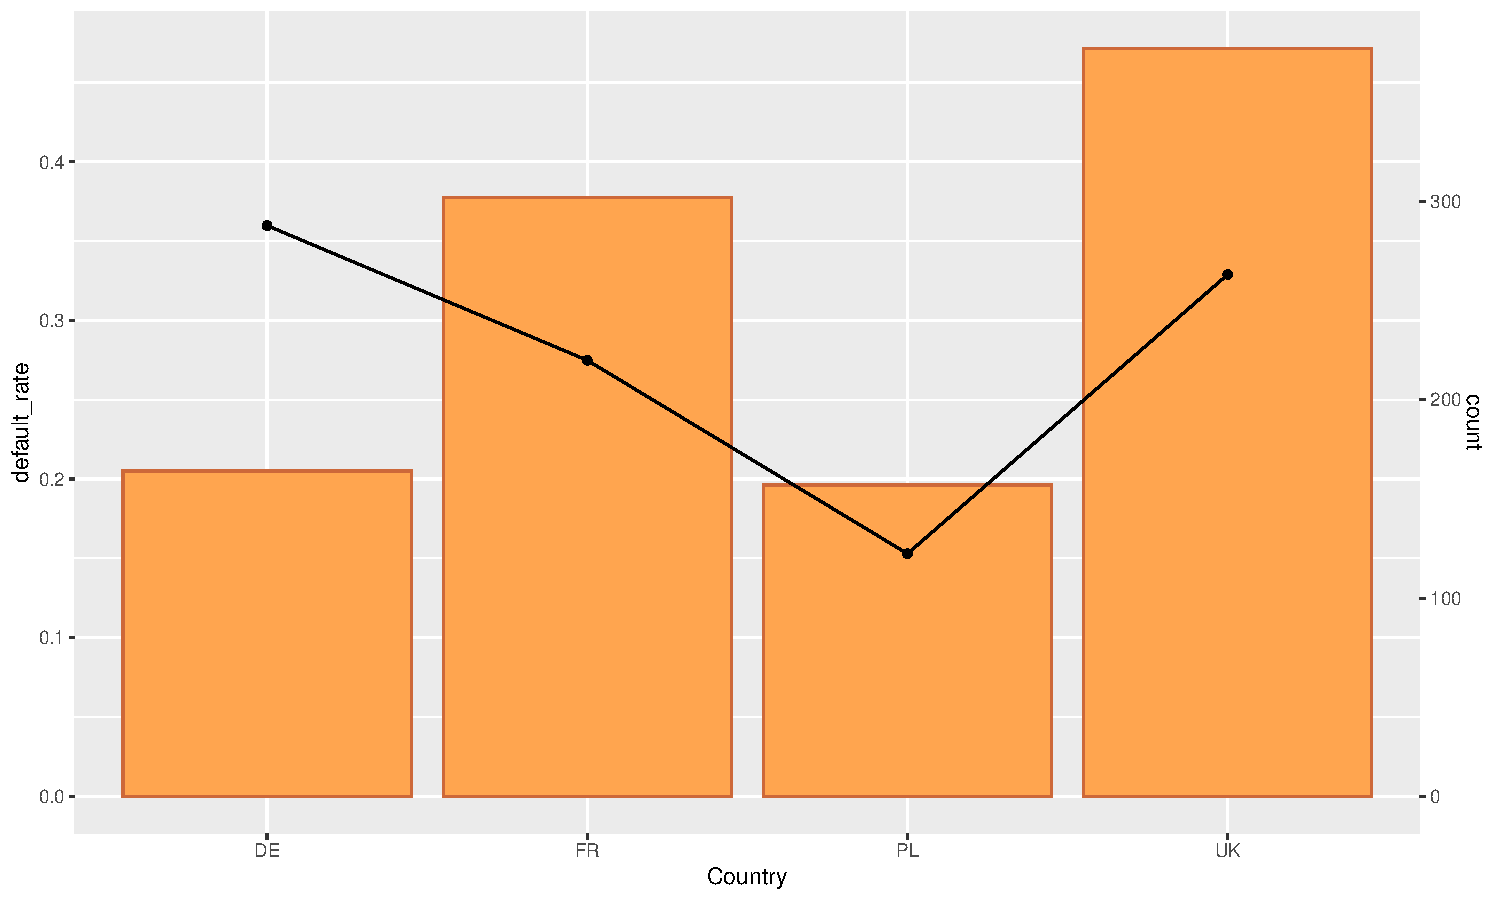
\includegraphics{Risk-Models-Development-Process_files/figure-beamer/unnamed-chunk-13-1.pdf}

\end{frame}

\begin{frame}{Single Factor Analysis - Bivariate - Country}

\begin{itemize}
\tightlist
\item
  Switch from categorical variable Country to boolean Country\_PL
\item
  Is this in line with common sense and expectations?
\item
  What is the expected impact of the variable on the final model?
\end{itemize}

\end{frame}

\begin{frame}[fragile]{Single Factor Analysis - Bivariate - Country}

\begin{Shaded}
\begin{Highlighting}[]
\NormalTok{Drivers_}\DecValTok{2}\NormalTok{ <-}\StringTok{ }\NormalTok{Drivers_}\DecValTok{1}
\NormalTok{Drivers_}\DecValTok{2}\OperatorTok{$}\NormalTok{Country_PL <-}\StringTok{ }\NormalTok{(Drivers_}\DecValTok{1}\OperatorTok{$}\NormalTok{Country }\OperatorTok{==}\StringTok{ "PL"}\NormalTok{)}\OperatorTok{*}\DecValTok{1}
\end{Highlighting}
\end{Shaded}

\end{frame}

\begin{frame}[fragile]{Single Factor Analysis - Bivariate - Country}

\begin{verbatim}
##  Country Industry Length_of_business Total_assets
##       UK        A                4.3          1.5
##       UK        D                8.7          9.8
##       FR        A                7.1          1.7
##       FR        A                5.6          6.2
##       UK        A                2.3         15.9
##       UK        B                4.1          7.3
##       PL        A                3.2          4.2
##  Credit_limit   EDF GDP_growth Default Country_PL
##          0.27 0.013       2.95       1          0
##          1.27 0.015       1.64       0          0
##          0.59 0.010       1.72       0          0
##          0.87 0.013       0.96       1          0
##          1.87 0.018       1.45       0          0
##          0.73 0.018       1.45       1          0
##          0.66 0.013       3.32       0          1
\end{verbatim}

\end{frame}

\begin{frame}[fragile]{Single Factor Analysis - Bivariate - Country}

We remove the variable Country now

\begin{Shaded}
\begin{Highlighting}[]
\NormalTok{Drivers_}\DecValTok{2}\NormalTok{ <-}\StringTok{ }\KeywordTok{subset}\NormalTok{(Drivers_}\DecValTok{2}\NormalTok{, }\DataTypeTok{select=}\OperatorTok{-}\KeywordTok{c}\NormalTok{(Country))}
\KeywordTok{print}\NormalTok{(}\KeywordTok{head}\NormalTok{(Drivers_}\DecValTok{2}\NormalTok{,}\DecValTok{7}\NormalTok{), }\DataTypeTok{digits =} \DecValTok{2}\NormalTok{, }\DataTypeTok{row.names =} \OtherTok{FALSE}\NormalTok{)}
\end{Highlighting}
\end{Shaded}

\end{frame}

\begin{frame}[fragile]{Single Factor Analysis - Bivariate - Country}

We remove the variable Country now

\begin{verbatim}
##   Industry Length_of_business Total_assets Credit_limit
## 1        A                4.3          1.5         0.27
## 2        D                8.7          9.8         1.27
## 3        A                7.1          1.7         0.59
## 4        A                5.6          6.2         0.87
## 5        A                2.3         15.9         1.87
## 6        B                4.1          7.3         0.73
## 7        A                3.2          4.2         0.66
##     EDF GDP_growth Default Country_PL
## 1 0.013       2.95       1          0
## 2 0.015       1.64       0          0
## 3 0.010       1.72       0          0
## 4 0.013       0.96       1          0
## 5 0.018       1.45       0          0
## 6 0.018       1.45       1          0
## 7 0.013       3.32       0          1
\end{verbatim}

\end{frame}

\begin{frame}[fragile]{Single Factor Analysis - Bivariate - Industry}

\begin{Shaded}
\begin{Highlighting}[]
\NormalTok{industry_group <-}\StringTok{ }\NormalTok{Data }\OperatorTok\StringTok{ }\KeywordTok{group_by}\NormalTok{(Industry) }\OperatorTok
\StringTok{  }\KeywordTok{summarise}\NormalTok{(}\DataTypeTok{default_rate =} \KeywordTok{mean}\NormalTok{(Default),}\DataTypeTok{count =} \KeywordTok{n}\NormalTok{())}
\KeywordTok{print}\NormalTok{(industry_group, }\DataTypeTok{digits =} \DecValTok{3}\NormalTok{, }\DataTypeTok{row.names =} \OtherTok{FALSE}\NormalTok{)}
\end{Highlighting}
\end{Shaded}

\begin{verbatim}
## # A tibble: 4 x 3
##   Industry default_rate count
##   <fct>           <dbl> <int>
## 1 A               0.349   387
## 2 B               0.415   106
## 3 C               0.236   292
## 4 D               0.195   215
\end{verbatim}

\end{frame}

\begin{frame}[fragile]{Single Factor Analysis - Bivariate - Industry}

\begin{Shaded}
\begin{Highlighting}[]
\KeywordTok{ggplot}\NormalTok{(}\DataTypeTok{data=}\NormalTok{industry_group, }\KeywordTok{aes}\NormalTok{(}\DataTypeTok{x=}\NormalTok{Industry, }\DataTypeTok{y=}\NormalTok{default_rate,}
                                \DataTypeTok{group=}\DecValTok{1}\NormalTok{)) }\OperatorTok{+}
\StringTok{    }\KeywordTok{geom_bar}\NormalTok{(}\KeywordTok{aes}\NormalTok{(}\DataTypeTok{x=}\NormalTok{Industry, }\DataTypeTok{y=}\NormalTok{count}\OperatorTok{/}\DecValTok{800}\NormalTok{),}\DataTypeTok{stat=}\StringTok{"identity"}\NormalTok{,}
             \DataTypeTok{fill=}\StringTok{"tan1"}\NormalTok{, }\DataTypeTok{colour=}\StringTok{"sienna3"}\NormalTok{)}\OperatorTok{+}
\StringTok{    }\KeywordTok{geom_line}\NormalTok{() }\OperatorTok{+}
\StringTok{    }\KeywordTok{geom_point}\NormalTok{()}\OperatorTok{+}
\StringTok{    }\KeywordTok{scale_y_continuous}\NormalTok{(}\DataTypeTok{name =} \KeywordTok{waiver}\NormalTok{(),}
                       \DataTypeTok{sec.axis =} \KeywordTok{sec_axis}\NormalTok{(}\OperatorTok{~}\StringTok{ }\NormalTok{. }\OperatorTok{*}\StringTok{ }\DecValTok{800}\NormalTok{,}
                                           \DataTypeTok{name =} \StringTok{"count"}\NormalTok{))}
\end{Highlighting}
\end{Shaded}

\end{frame}

\begin{frame}{Single Factor Analysis - Bivariate - Industry}

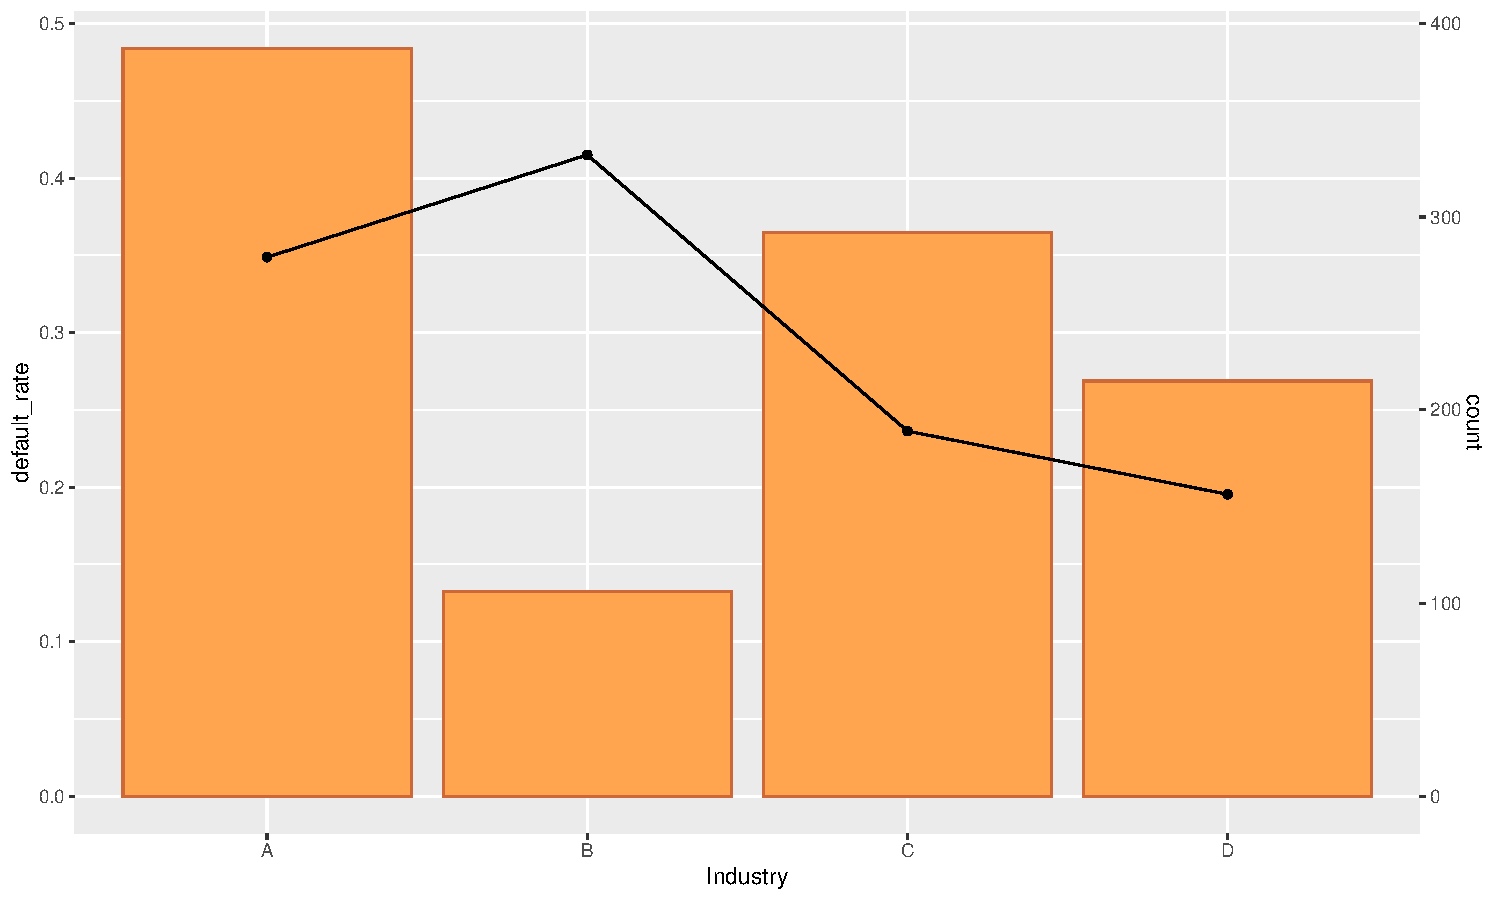
\includegraphics{Risk-Models-Development-Process_files/figure-beamer/unnamed-chunk-20-1.pdf}

\end{frame}

\begin{frame}{Single Factor Analysis - Bivariate - Industry}

\begin{itemize}
\tightlist
\item
  Switch from categorical variables Industry \(\in\) \{A, B\} to boolean
  Industry\_AB
\item
  Is this in line with common sense and expectations?
\item
  What is the expected impact of the variable on the final model?
\end{itemize}

\end{frame}

\begin{frame}[fragile]{Single Factor Analysis - Bivariate - Industry}

\begin{Shaded}
\begin{Highlighting}[]
\NormalTok{Drivers_}\DecValTok{3}\NormalTok{ <-}\StringTok{ }\NormalTok{Drivers_}\DecValTok{2}
\NormalTok{Drivers_}\DecValTok{3}\OperatorTok{$}\NormalTok{Industry_AB <-}\StringTok{ }\NormalTok{(Drivers_}\DecValTok{2}\OperatorTok{$}\NormalTok{Industry }\OperatorTok\StringTok{ }\KeywordTok{c}\NormalTok{(}\StringTok{"A"}\NormalTok{,}\StringTok{"B"}\NormalTok{))}\OperatorTok{*}\DecValTok{1}
\KeywordTok{print}\NormalTok{(}\KeywordTok{head}\NormalTok{(}\KeywordTok{subset}\NormalTok{(Drivers_}\DecValTok{3}\NormalTok{, }\DataTypeTok{select=}\OperatorTok{-}\KeywordTok{c}\NormalTok{(Customer_ID)),}\DecValTok{7}\NormalTok{),}
      \DataTypeTok{digits =} \DecValTok{2}\NormalTok{, }\DataTypeTok{row.names =} \OtherTok{FALSE}\NormalTok{)}
\end{Highlighting}
\end{Shaded}

\end{frame}

\begin{frame}[fragile]{Single Factor Analysis - Bivariate - Industry}

\begin{verbatim}
##  Industry Length_of_business Total_assets Credit_limit
##         A                4.3          1.5         0.27
##         D                8.7          9.8         1.27
##         A                7.1          1.7         0.59
##         A                5.6          6.2         0.87
##         A                2.3         15.9         1.87
##         B                4.1          7.3         0.73
##         A                3.2          4.2         0.66
##    EDF GDP_growth Default Country_PL Industry_AB
##  0.013       2.95       1          0           1
##  0.015       1.64       0          0           0
##  0.010       1.72       0          0           1
##  0.013       0.96       1          0           1
##  0.018       1.45       0          0           1
##  0.018       1.45       1          0           1
##  0.013       3.32       0          1           1
\end{verbatim}

\end{frame}

\begin{frame}[fragile]{Single Factor Analysis - Bivariate - Industry}

\begin{verbatim}
##  Length_of_business Total_assets Credit_limit   EDF
##                 4.3          1.5         0.27 0.013
##                 8.7          9.8         1.27 0.015
##                 7.1          1.7         0.59 0.010
##                 5.6          6.2         0.87 0.013
##                 2.3         15.9         1.87 0.018
##                 4.1          7.3         0.73 0.018
##                 3.2          4.2         0.66 0.013
##  GDP_growth Default Country_PL Industry_AB
##        2.95       1          0           1
##        1.64       0          0           0
##        1.72       0          0           1
##        0.96       1          0           1
##        1.45       0          0           1
##        1.45       1          0           1
##        3.32       0          1           1
\end{verbatim}

\end{frame}

\begin{frame}[fragile]{Single Factor Analysis - Bivariate -
Length\_of\_business}

Let's bucket the data by year

\begin{verbatim}
## # A tibble: 19 x 3
##    Length_of_business_Floor default_rate count
##                       <dbl>        <dbl> <int>
##  1                        0       0.469     32
##  2                        1       0.459    111
##  3                        2       0.377    167
##  4                        3       0.384    151
##  5                        4       0.271    140
##  6                        5       0.266    109
##  7                        6       0.2       85
##  8                        7       0.138     58
##  9                        8       0.1       50
## 10                        9       0.121     33
## 11                       10       0.0714    14
## 12                       11       0         13
## 13                       12       0         12
## 14                       13       0.167      6
## 15                       14       0          7
## 16                       15       0          5
## 17                       16       0          3
## 18                       18       0          2
## 19                       20       0          2
\end{verbatim}

\end{frame}

\begin{frame}[fragile]{Single Factor Analysis - Bivariate -
Length\_of\_business}

Let's cut the dataset in 11 and put everything longer than that into one
group

\begin{verbatim}
## # A tibble: 12 x 3
##    Length_of_business_Floor default_rate count
##                       <dbl>        <dbl> <int>
##  1                        0       0.469     32
##  2                        1       0.459    111
##  3                        2       0.377    167
##  4                        3       0.384    151
##  5                        4       0.271    140
##  6                        5       0.266    109
##  7                        6       0.2       85
##  8                        7       0.138     58
##  9                        8       0.1       50
## 10                        9       0.121     33
## 11                       10       0.0714    14
## 12                       11       0.02      50
\end{verbatim}

\end{frame}

\begin{frame}[fragile]{Single Factor Analysis - Bivariate -
Length\_of\_business}

\begin{Shaded}
\begin{Highlighting}[]
\KeywordTok{ggplot}\NormalTok{(}\DataTypeTok{data=}\NormalTok{length_group, }\KeywordTok{aes}\NormalTok{(}\DataTypeTok{x=}\NormalTok{Length_of_business_Floor,}
                              \DataTypeTok{y=}\NormalTok{default_rate, }\DataTypeTok{group=}\DecValTok{1}\NormalTok{)) }\OperatorTok{+}
\StringTok{    }\KeywordTok{geom_bar}\NormalTok{(}\KeywordTok{aes}\NormalTok{(}\DataTypeTok{x=}\NormalTok{Length_of_business_Floor, }\DataTypeTok{y=}\NormalTok{count}\OperatorTok{/}\DecValTok{400}\NormalTok{),}
             \DataTypeTok{stat=}\StringTok{"identity"}\NormalTok{,}
             \DataTypeTok{fill=}\StringTok{"tan1"}\NormalTok{, }\DataTypeTok{colour=}\StringTok{"sienna3"}\NormalTok{)}\OperatorTok{+}
\StringTok{    }\KeywordTok{geom_line}\NormalTok{() }\OperatorTok{+}
\StringTok{    }\KeywordTok{geom_point}\NormalTok{()}\OperatorTok{+}
\StringTok{    }\KeywordTok{scale_y_continuous}\NormalTok{(}\DataTypeTok{name =} \KeywordTok{waiver}\NormalTok{(),}
                       \DataTypeTok{sec.axis =} \KeywordTok{sec_axis}\NormalTok{(}\OperatorTok{~}\StringTok{ }\NormalTok{. }\OperatorTok{*}\StringTok{ }\DecValTok{400}\NormalTok{,}
                                           \DataTypeTok{name =} \StringTok{"count"}\NormalTok{))}
\end{Highlighting}
\end{Shaded}

\end{frame}

\begin{frame}{Single Factor Analysis - Bivariate - Length\_of\_business}

\begin{itemize}
\tightlist
\item
  Is this relation in line with logic?
  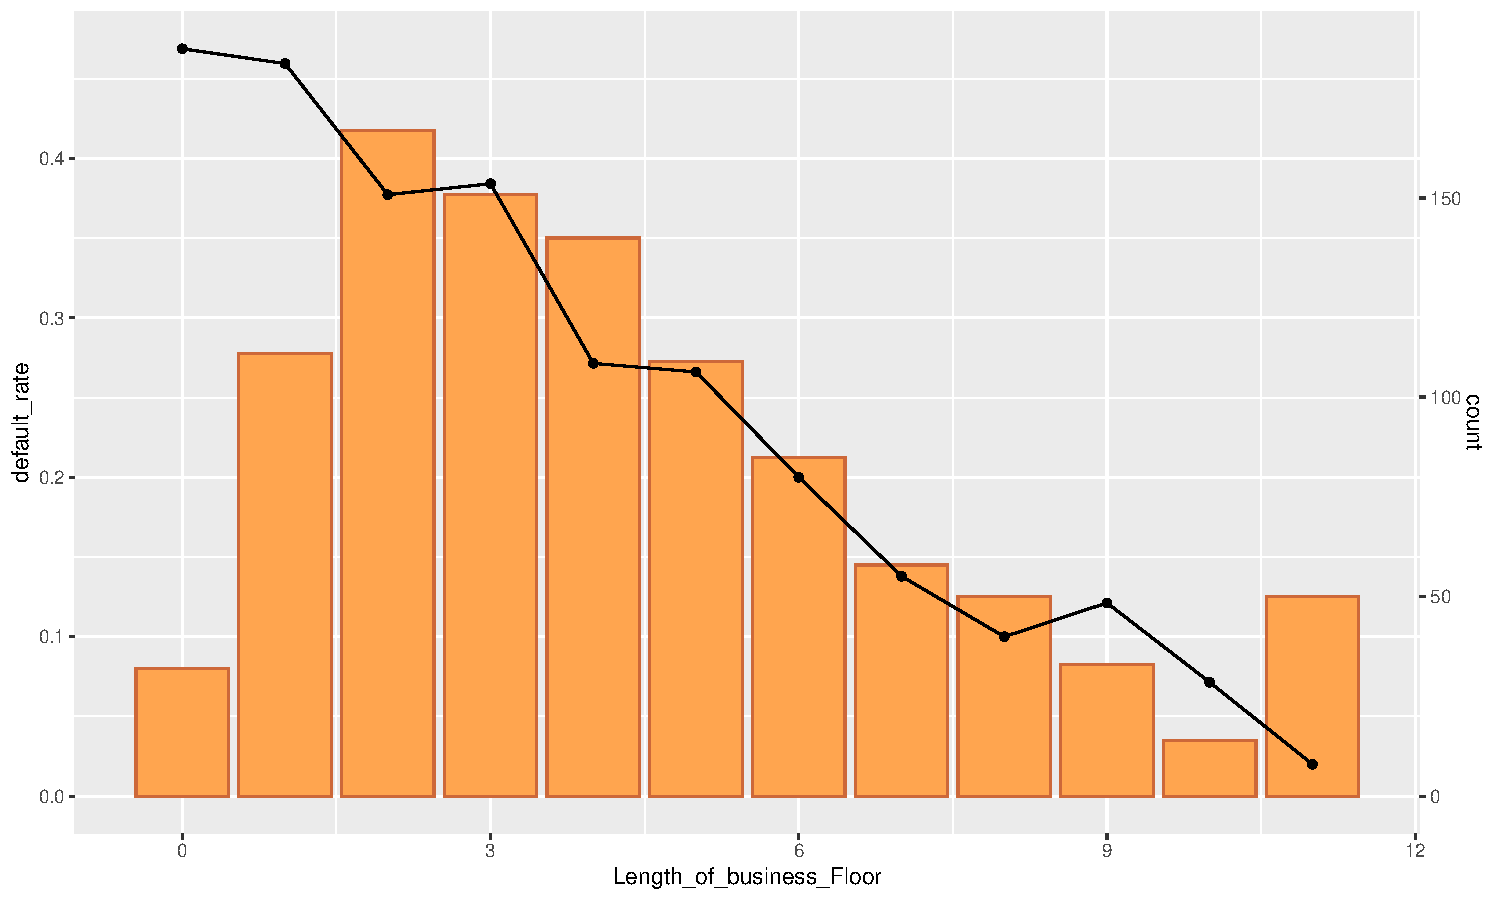
\includegraphics{Risk-Models-Development-Process_files/figure-beamer/unnamed-chunk-27-1.pdf}
\end{itemize}

\end{frame}

\begin{frame}[fragile]{Single Factor Analysis - Bivariate -
Total\_assets}

\begin{Shaded}
\begin{Highlighting}[]
\NormalTok{Data}\OperatorTok{$}\NormalTok{Total_assets_Floor <-}\StringTok{ }\KeywordTok{floor}\NormalTok{(Data}\OperatorTok{$}\NormalTok{Total_assets)}
\NormalTok{assets_group <-}\StringTok{ }\NormalTok{Data }\OperatorTok\StringTok{ }\KeywordTok{group_by}\NormalTok{(}
\NormalTok{  Total_assets_Floor) }\OperatorTok\StringTok{ }\KeywordTok{summarise}\NormalTok{(}
    \DataTypeTok{default_rate =} \KeywordTok{mean}\NormalTok{(Default),}\DataTypeTok{count =} \KeywordTok{n}\NormalTok{())}
\KeywordTok{print}\NormalTok{(assets_group, }\DataTypeTok{digits =} \DecValTok{3}\NormalTok{, }\DataTypeTok{row.names =} \OtherTok{FALSE}\NormalTok{)}
\end{Highlighting}
\end{Shaded}

\end{frame}

\begin{frame}[fragile]{Single Factor Analysis - Bivariate -
Total\_assets}

\begin{verbatim}
## # A tibble: 16 x 3
##    Total_assets_Floor default_rate count
##                 <dbl>        <dbl> <int>
##  1                  0        0.320   181
##  2                  1        0.322   236
##  3                  2        0.304   184
##  4                  3        0.321   134
##  5                  4        0.207    87
##  6                  5        0.255    55
##  7                  6        0.268    41
##  8                  7        0.167    30
##  9                  8        0.15     20
## 10                  9        0.167     6
## 11                 10        0.167     6
## 12                 11        0.222     9
## 13                 12        0         4
## 14                 13        0.5       4
## 15                 14        0         1
## 16                 15        0         2
\end{verbatim}

\end{frame}

\begin{frame}[fragile]{Single Factor Analysis - Bivariate -
Total\_assets}

Let's cut the dataset in 8 and put everything longer than that into one
group

\begin{verbatim}
## # A tibble: 9 x 3
##   Total_assets_Floor default_rate count
##                <dbl>        <dbl> <int>
## 1                  0        0.320   181
## 2                  1        0.322   236
## 3                  2        0.304   184
## 4                  3        0.321   134
## 5                  4        0.207    87
## 6                  5        0.255    55
## 7                  6        0.268    41
## 8                  7        0.167    30
## 9                  8        0.173    52
\end{verbatim}

\end{frame}

\begin{frame}[fragile]{Single Factor Analysis - Bivariate -
Total\_assets}

\begin{Shaded}
\begin{Highlighting}[]
\KeywordTok{ggplot}\NormalTok{(}\DataTypeTok{data=}\NormalTok{assets_group, }\KeywordTok{aes}\NormalTok{(}\DataTypeTok{x=}\NormalTok{Total_assets_Floor, }\DataTypeTok{y=}\NormalTok{default_rate,}
                              \DataTypeTok{group=}\DecValTok{1}\NormalTok{)) }\OperatorTok{+}
\StringTok{    }\KeywordTok{geom_bar}\NormalTok{(}\KeywordTok{aes}\NormalTok{(}\DataTypeTok{x=}\NormalTok{Total_assets_Floor, }\DataTypeTok{y=}\NormalTok{count}\OperatorTok{/}\DecValTok{500}\NormalTok{),}
             \DataTypeTok{stat=}\StringTok{"identity"}\NormalTok{,}
             \DataTypeTok{fill=}\StringTok{"tan1"}\NormalTok{, }\DataTypeTok{colour=}\StringTok{"sienna3"}\NormalTok{)}\OperatorTok{+}
\StringTok{    }\KeywordTok{geom_line}\NormalTok{() }\OperatorTok{+}
\StringTok{    }\KeywordTok{geom_point}\NormalTok{()}\OperatorTok{+}
\StringTok{    }\KeywordTok{scale_y_continuous}\NormalTok{(}\DataTypeTok{name =} \KeywordTok{waiver}\NormalTok{(),}
                       \DataTypeTok{sec.axis =} \KeywordTok{sec_axis}\NormalTok{(}\OperatorTok{~}\StringTok{ }\NormalTok{. }\OperatorTok{*}\StringTok{ }\DecValTok{500}\NormalTok{,}
                                           \DataTypeTok{name =} \StringTok{"count"}\NormalTok{))}
\end{Highlighting}
\end{Shaded}

\end{frame}

\begin{frame}{Single Factor Analysis - Bivariate - Total\_assets}

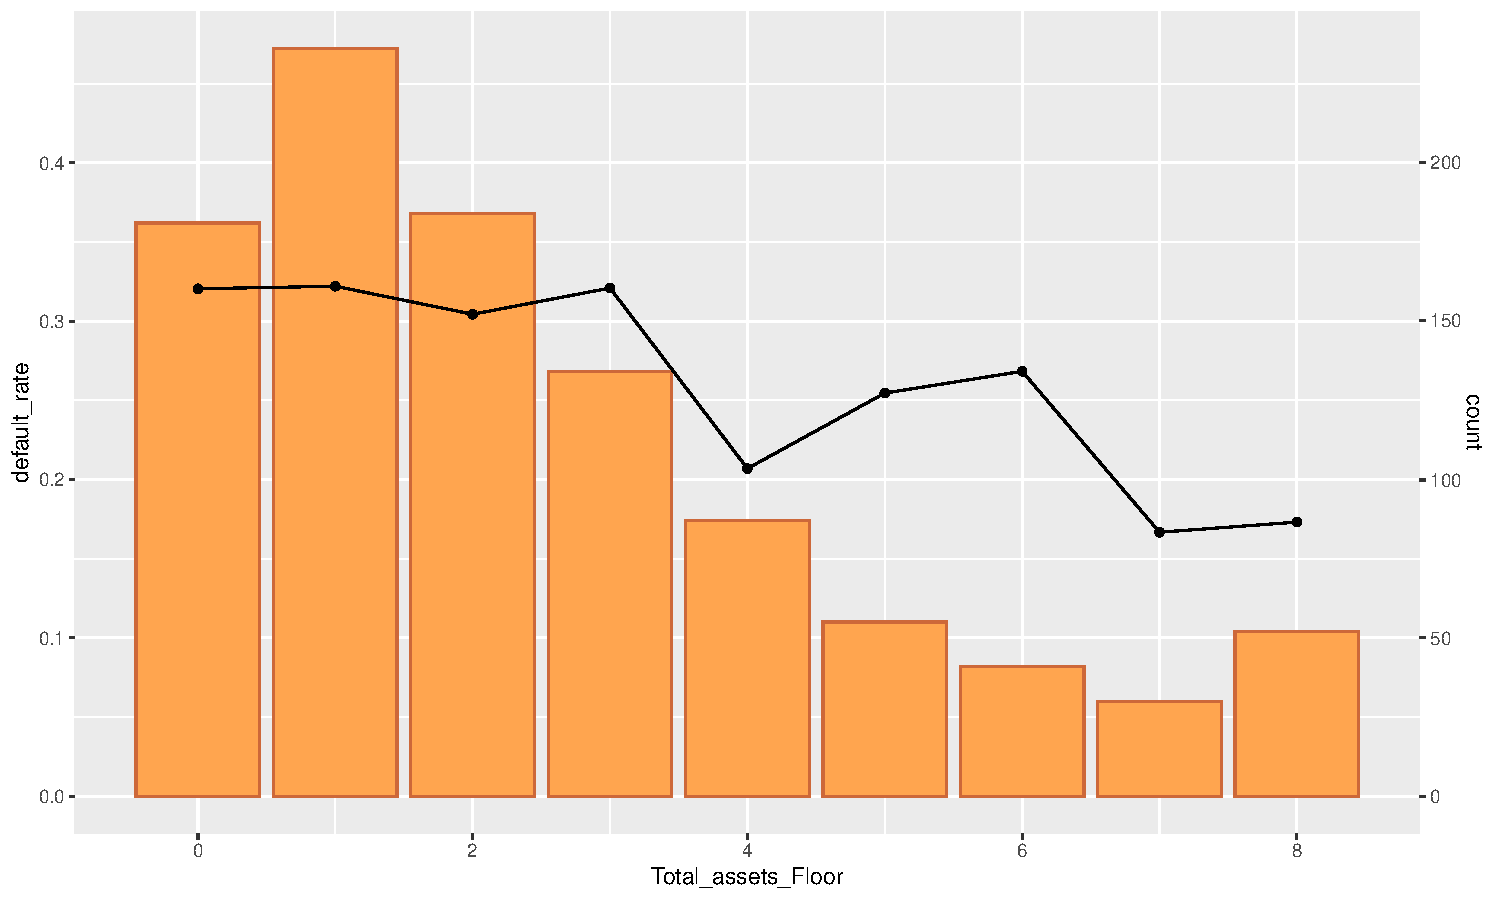
\includegraphics{Risk-Models-Development-Process_files/figure-beamer/unnamed-chunk-32-1.pdf}

\end{frame}

\begin{frame}[fragile]{Single Factor Analysis - Bivariate -
Credit\_limit}

\begin{verbatim}
## # A tibble: 6 x 3
##   Credit_limit_Floor default_rate count
##                <dbl>        <dbl> <int>
## 1               0           0.290   107
## 2               0.25        0.303   350
## 3               0.5         0.312   266
## 4               0.75        0.266   143
## 5               1           0.265    68
## 6               1.25        0.212    66
\end{verbatim}

\end{frame}

\begin{frame}{Single Factor Analysis - Bivariate - Credit\_limit}

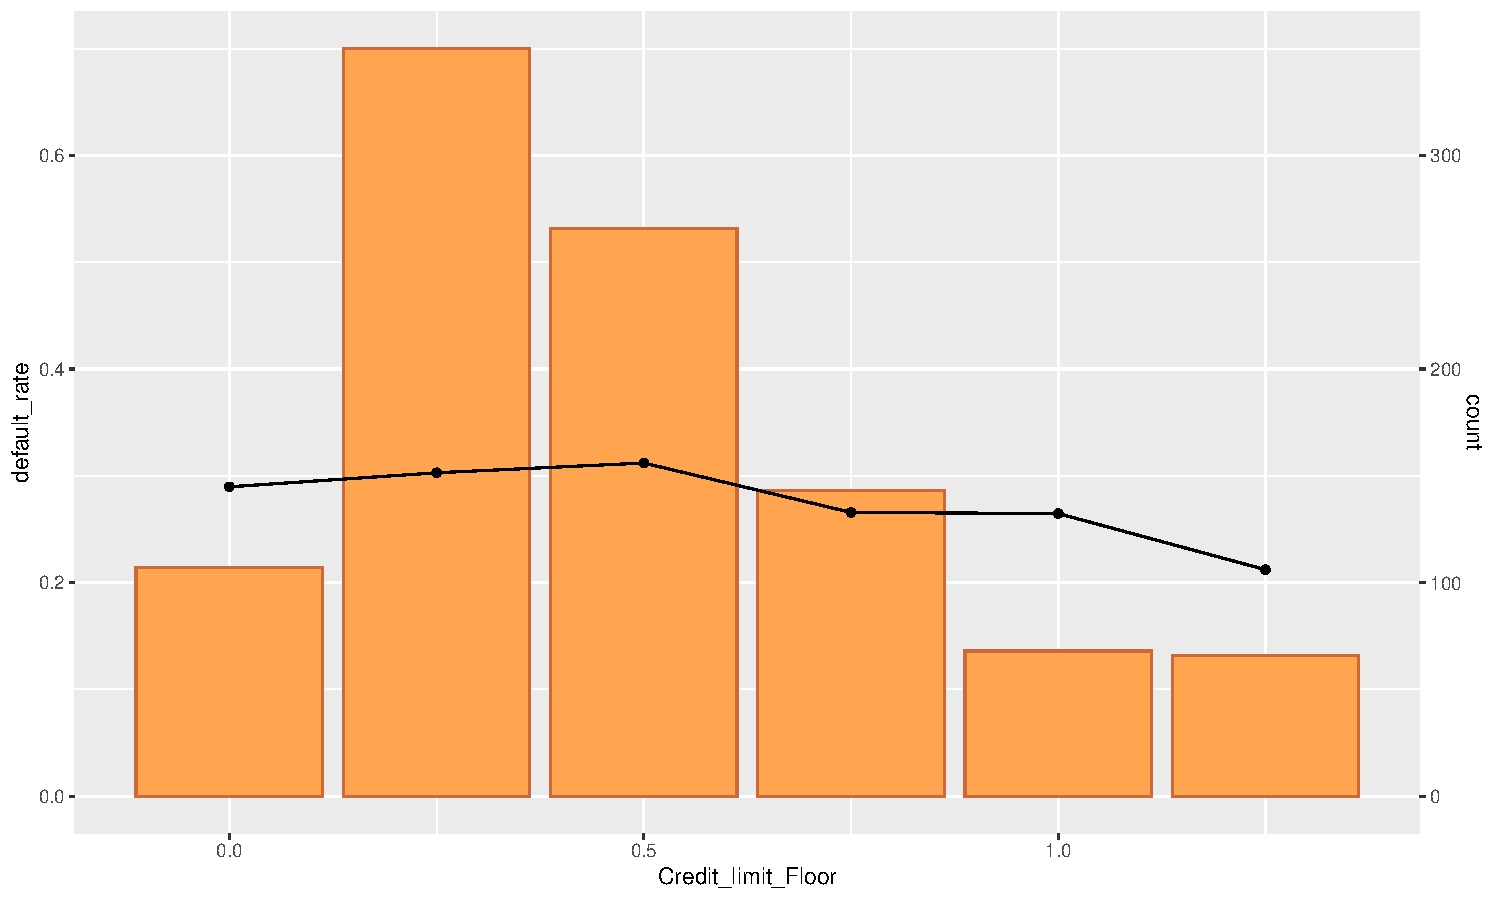
\includegraphics{Risk-Models-Development-Process_files/figure-beamer/unnamed-chunk-35-1.pdf}

\end{frame}

\begin{frame}[fragile]{Single Factor Analysis - Bivariate - Expected
Default Frequency}

EDF is a variable common to all debtors dependent on year

\begin{Shaded}
\begin{Highlighting}[]
\NormalTok{EDF_group <-}\StringTok{ }\NormalTok{Data }\OperatorTok\StringTok{ }\KeywordTok{group_by}\NormalTok{(Date_of_data) }\OperatorTok
\StringTok{  }\KeywordTok{summarise}\NormalTok{(}\DataTypeTok{default_rate =} \KeywordTok{mean}\NormalTok{(Default), }\DataTypeTok{EDF =} \KeywordTok{mean}\NormalTok{(EDF),}
            \DataTypeTok{count =} \KeywordTok{n}\NormalTok{())}
\KeywordTok{print}\NormalTok{(EDF_group, }\DataTypeTok{digits =} \DecValTok{3}\NormalTok{, }\DataTypeTok{row.names =} \OtherTok{FALSE}\NormalTok{)}
\end{Highlighting}
\end{Shaded}

\begin{verbatim}
## # A tibble: 8 x 4
##   Date_of_data default_rate    EDF count
##   <fct>               <dbl>  <dbl> <int>
## 1 01/01/2011          0.291 0.015    110
## 2 01/01/2012          0.363 0.018    135
## 3 01/01/2013          0.262 0.021    145
## 4 01/01/2014          0.257 0.013    144
## 5 01/01/2015          0.301 0.0116    93
## 6 01/01/2016          0.3   0.0121   110
## 7 01/01/2017          0.275 0.0099   120
## 8 01/01/2018          0.280 0.0102   143
\end{verbatim}

\end{frame}

\begin{frame}{Single Factor Analysis - Bivariate - Expected Default
Frequency}

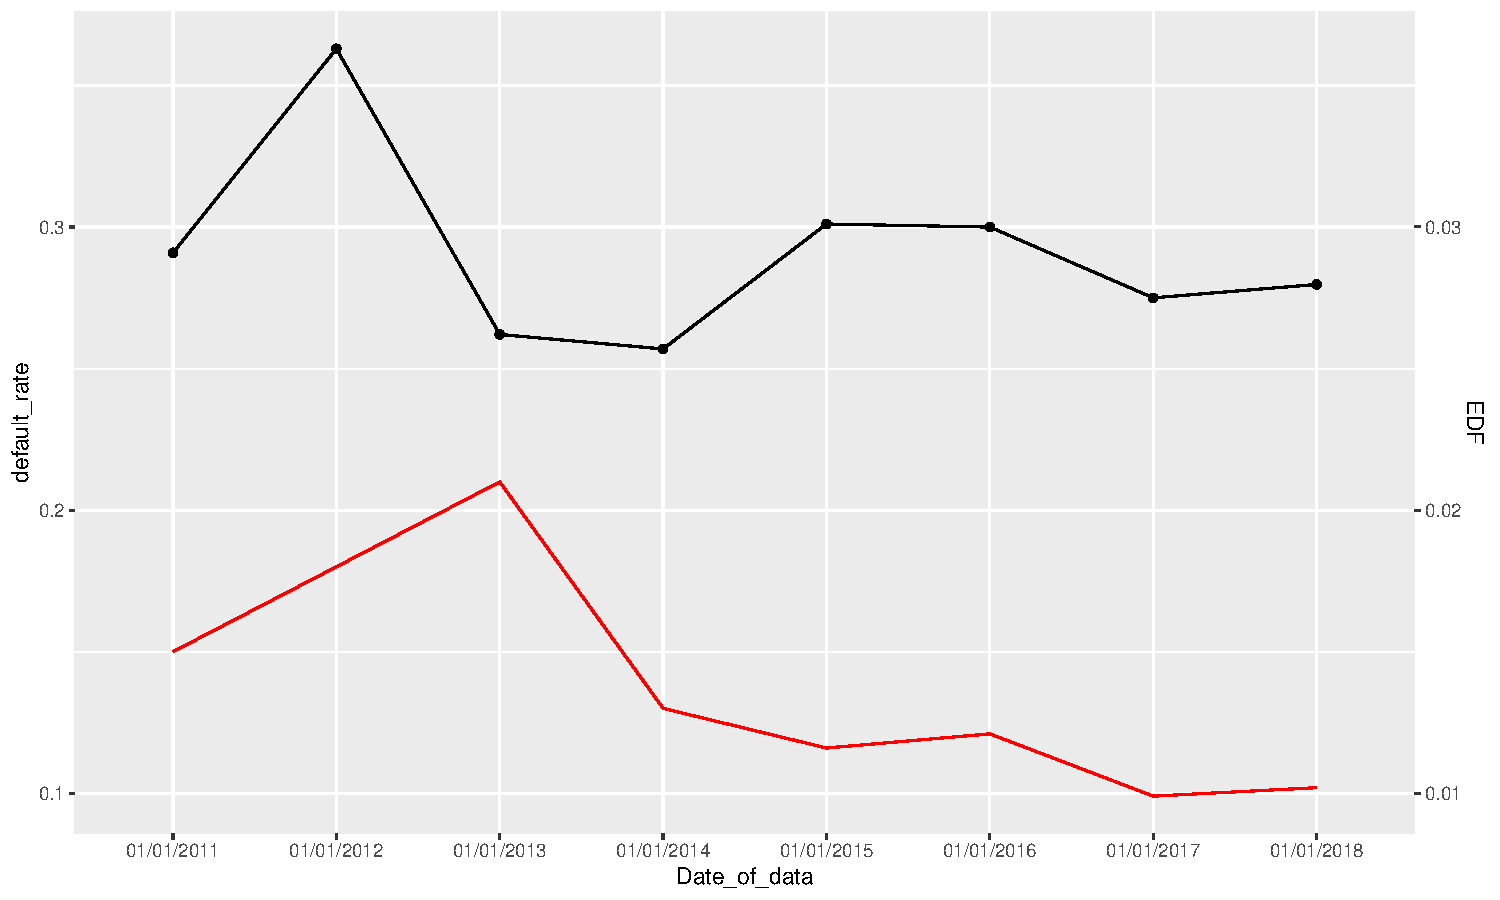
\includegraphics{Risk-Models-Development-Process_files/figure-beamer/unnamed-chunk-37-1.pdf}

\end{frame}

\begin{frame}[fragile]{Single Factor Analysis - Bivariate - Expected
Default Frequency}

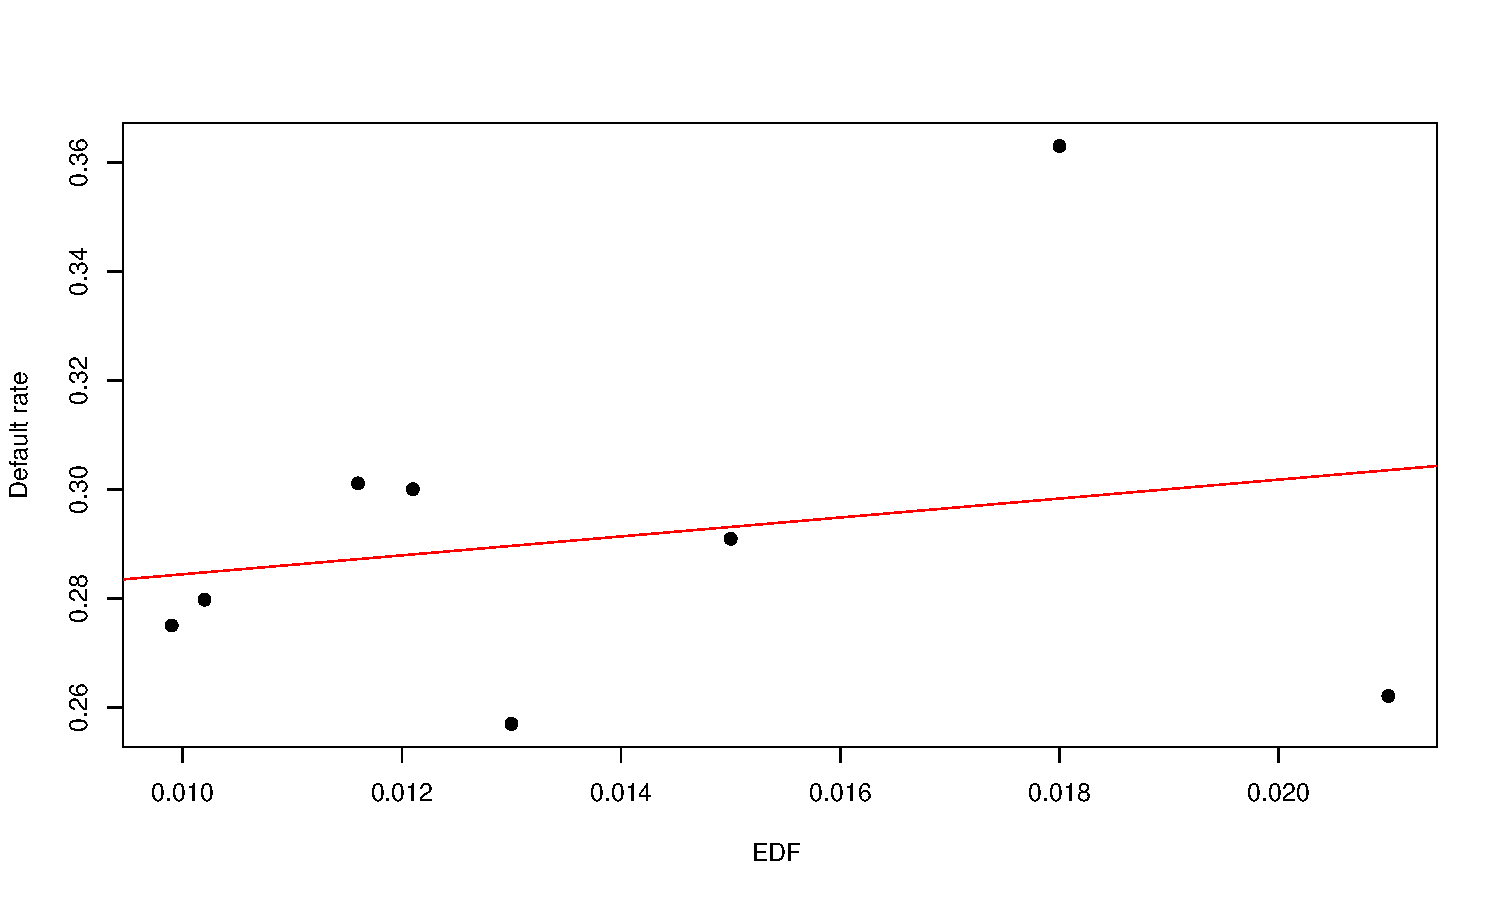
\includegraphics{Risk-Models-Development-Process_files/figure-beamer/unnamed-chunk-38-1.pdf}

\begin{verbatim}
## integer(0)
\end{verbatim}

\end{frame}

\begin{frame}[fragile]{Single Factor Analysis - Bivariate - GDP\_growth}

GDP\_growth is a variable common to all debtors dependent on year and
country

\begin{Shaded}
\begin{Highlighting}[]
\NormalTok{GDP_group <-}\StringTok{ }\NormalTok{Data }\OperatorTok\StringTok{ }\KeywordTok{group_by}\NormalTok{(Date_of_data,Country) }\OperatorTok
\StringTok{  }\KeywordTok{summarise}\NormalTok{(}\DataTypeTok{default_rate =} \KeywordTok{mean}\NormalTok{(Default),}\DataTypeTok{GDP_growth =} \KeywordTok{mean}\NormalTok{(GDP_growth))}
\KeywordTok{print}\NormalTok{(GDP_group, }\DataTypeTok{digits =} \DecValTok{3}\NormalTok{, }\DataTypeTok{row.names =} \OtherTok{FALSE}\NormalTok{)}
\end{Highlighting}
\end{Shaded}

\begin{verbatim}
## # A tibble: 32 x 4
## # Groups:   Date_of_data [8]
##    Date_of_data Country default_rate GDP_growth
##    <fct>        <fct>          <dbl>      <dbl>
##  1 01/01/2011   DE            0.286       3.66 
##  2 01/01/2011   FR            0.302       2.19 
##  3 01/01/2011   PL            0.0909      5.02 
##  4 01/01/2011   UK            0.333       1.64 
##  5 01/01/2012   DE            0.474       0.49 
##  6 01/01/2012   FR            0.289       0.31 
##  7 01/01/2012   PL            0.294       1.61 
##  8 01/01/2012   UK            0.407       1.45 
##  9 01/01/2013   DE            0.381       0.49 
## 10 01/01/2013   FR            0.25        0.580
## # ... with 22 more rows
\end{verbatim}

\end{frame}

\begin{frame}{Single Factor Analysis - Bivariate - GDP\_growth - UK}

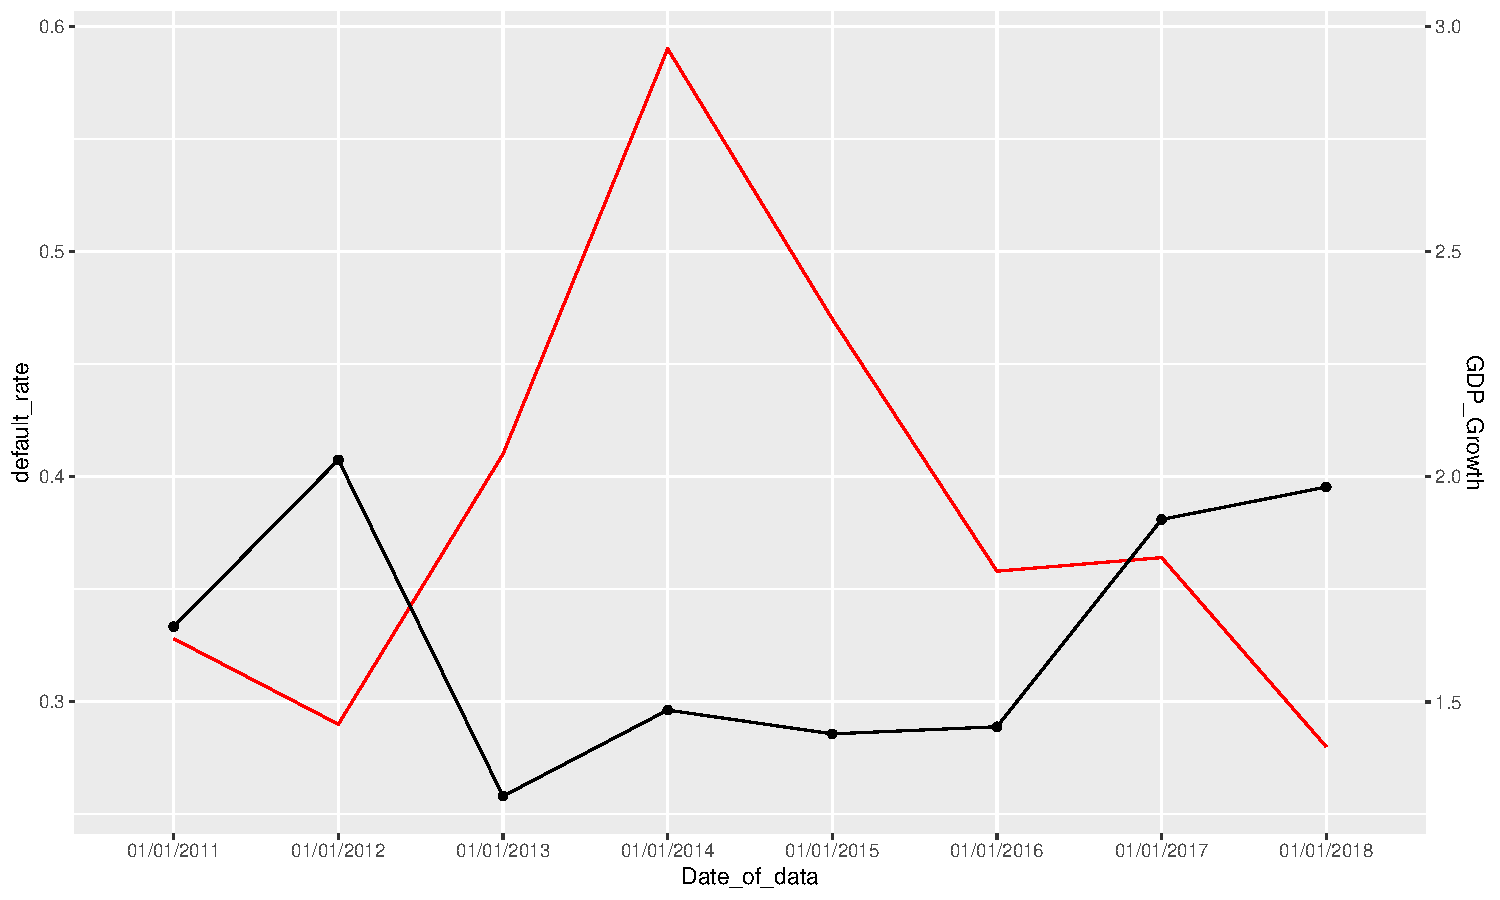
\includegraphics{Risk-Models-Development-Process_files/figure-beamer/unnamed-chunk-40-1.pdf}

\end{frame}

\begin{frame}{Single Factor Analysis - Bivariate - GDP\_growth - FR}

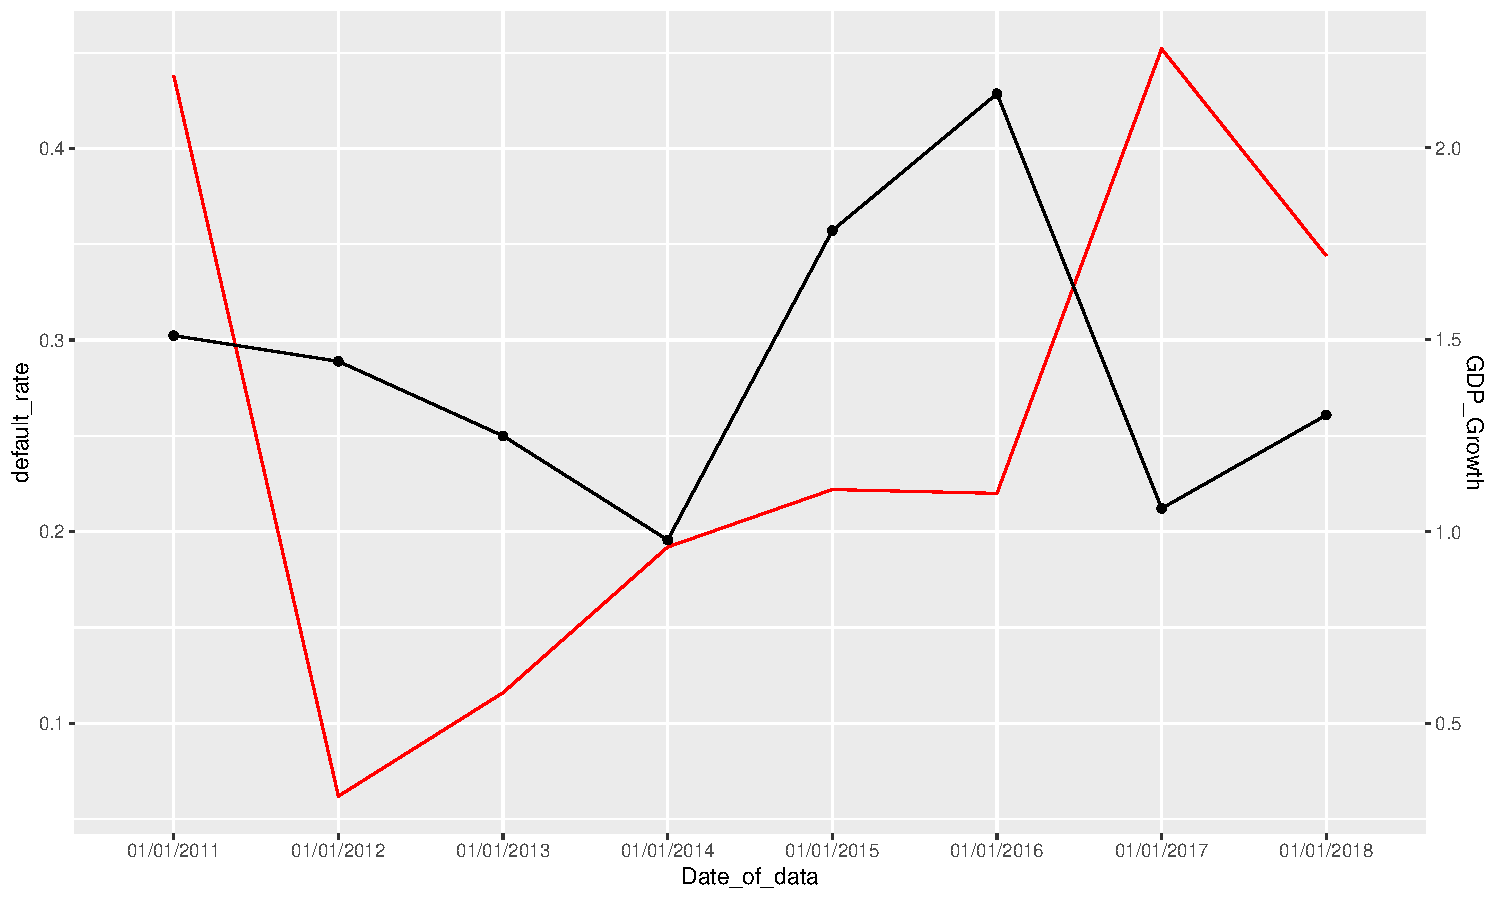
\includegraphics{Risk-Models-Development-Process_files/figure-beamer/unnamed-chunk-41-1.pdf}

\end{frame}

\begin{frame}{Single Factor Analysis - Bivariate - GDP\_growth - DE}

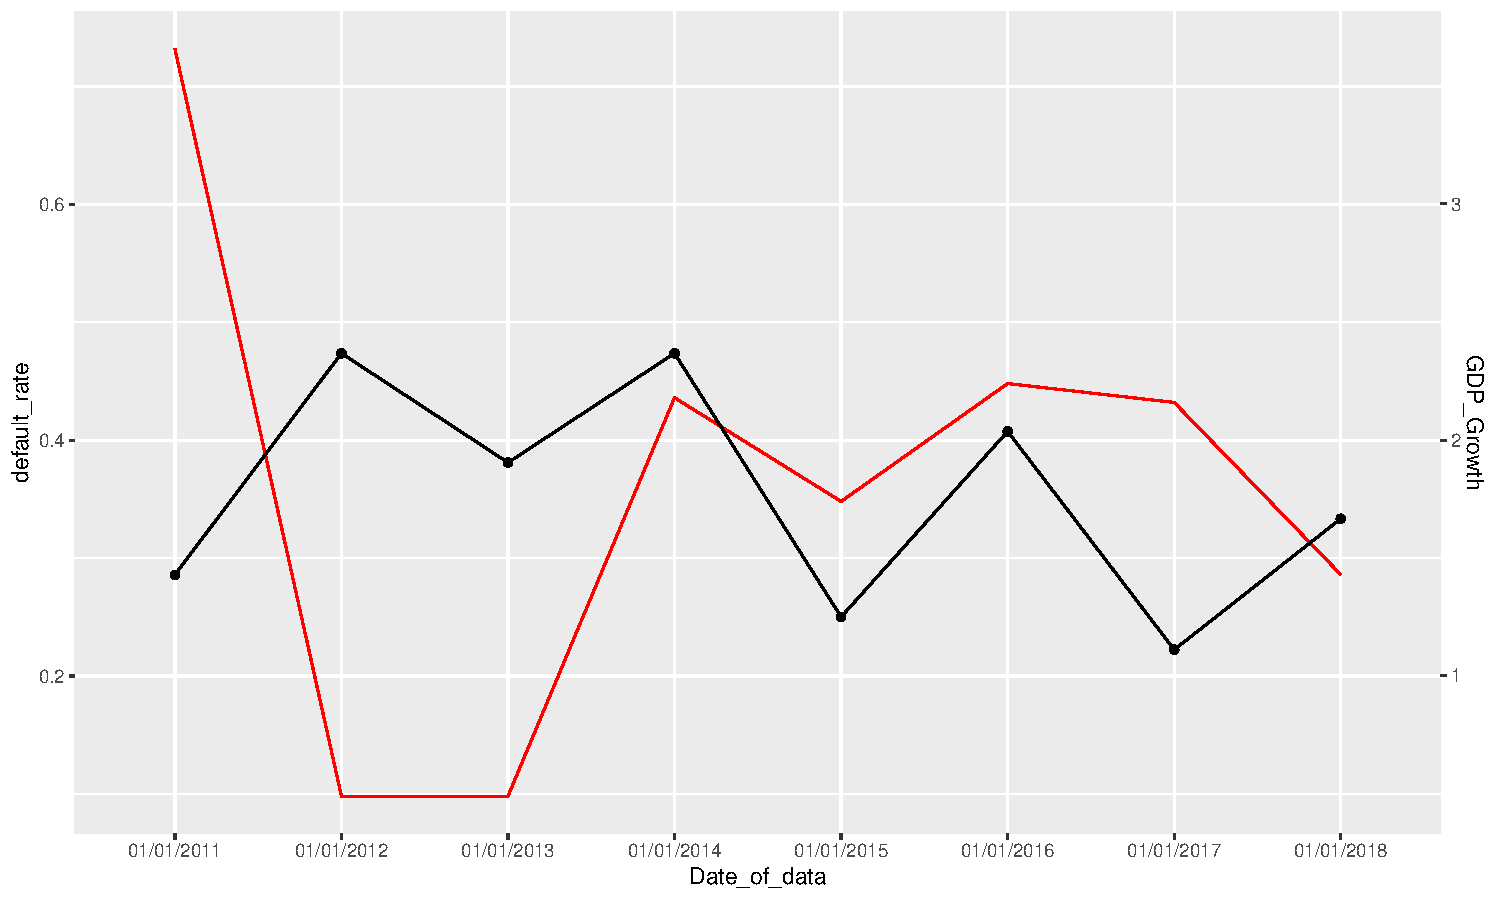
\includegraphics{Risk-Models-Development-Process_files/figure-beamer/unnamed-chunk-42-1.pdf}

\end{frame}

\begin{frame}{Single Factor Analysis - Bivariate - GDP\_growth - PL}

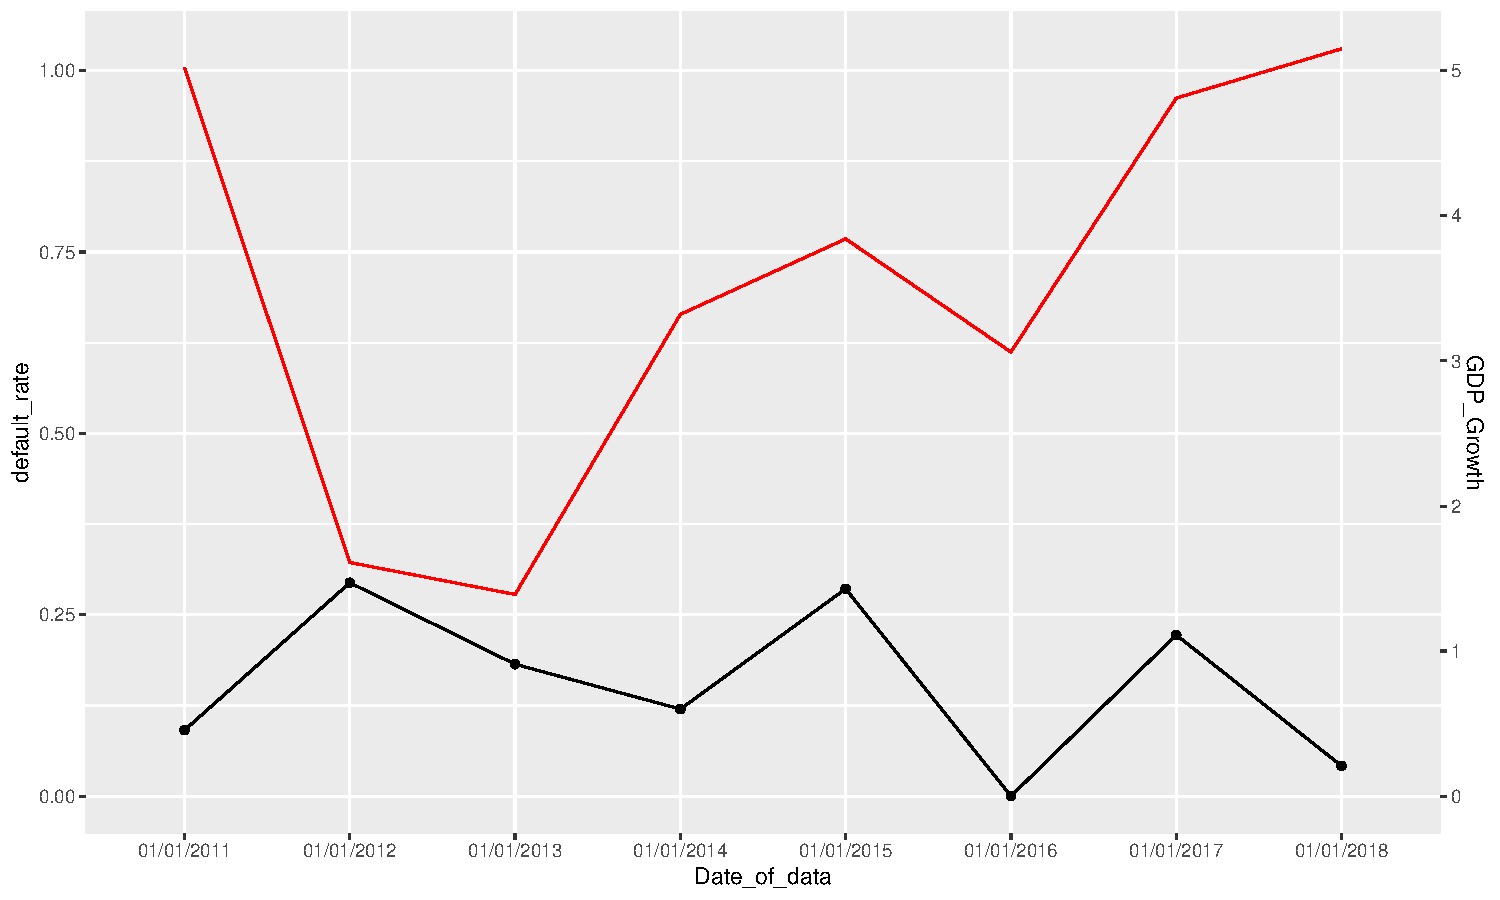
\includegraphics{Risk-Models-Development-Process_files/figure-beamer/unnamed-chunk-43-1.pdf}

\end{frame}

\begin{frame}[fragile]{Single Factor Analysis - Bivariate - GDP\_growth
- All countries}

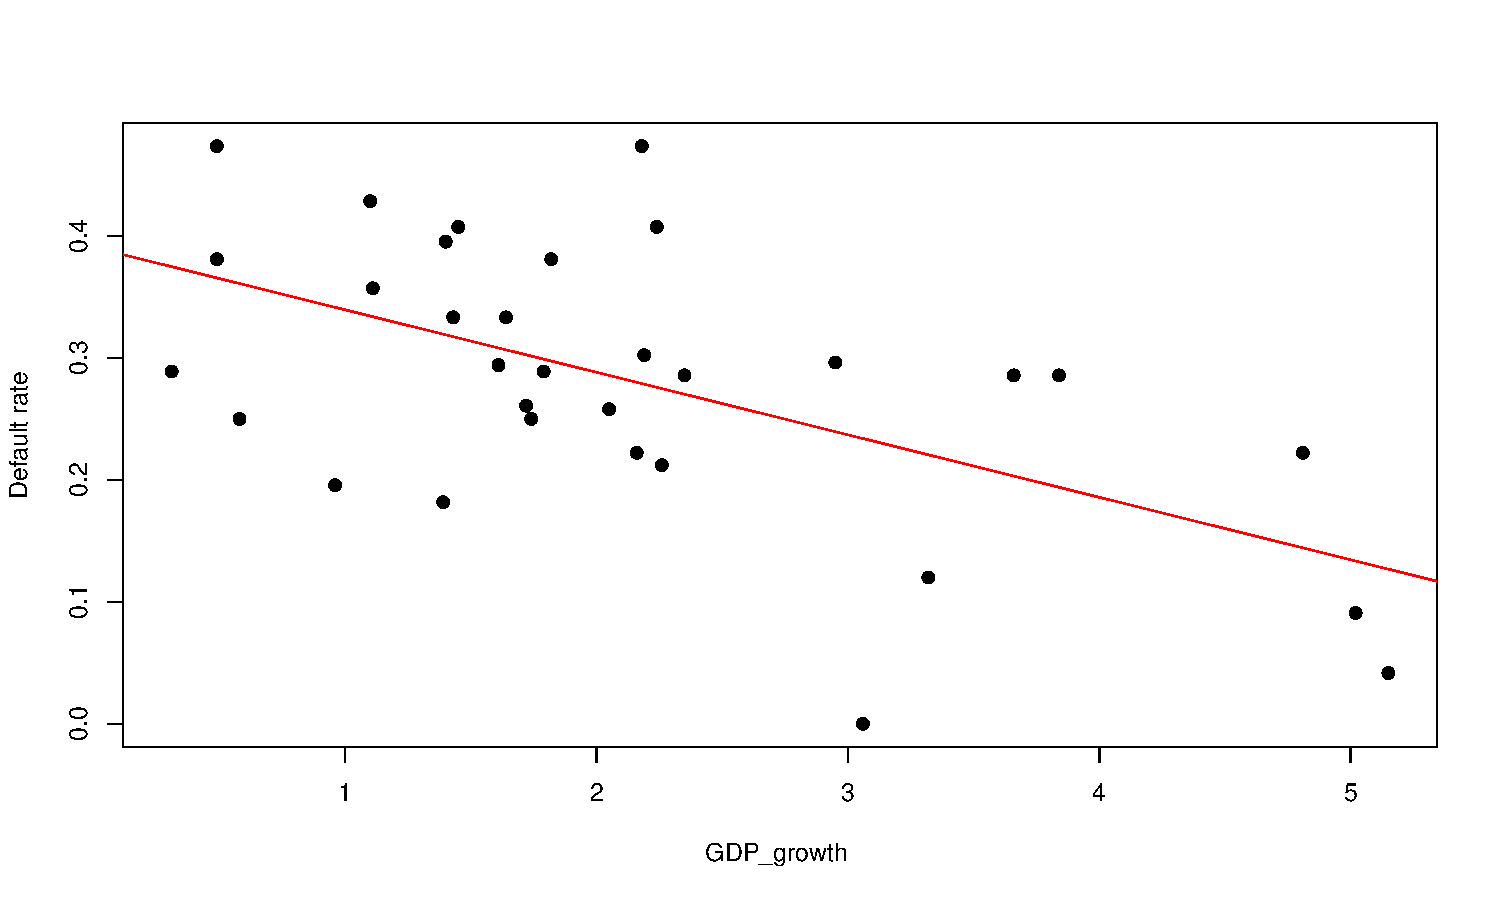
\includegraphics{Risk-Models-Development-Process_files/figure-beamer/unnamed-chunk-44-1.pdf}

\begin{verbatim}
## integer(0)
\end{verbatim}

\end{frame}

\begin{frame}[fragile]{Final dataset}

\begin{Shaded}
\begin{Highlighting}[]
\NormalTok{Drivers_final <-}\StringTok{ }\NormalTok{Drivers_}\DecValTok{3}\NormalTok{[, }\KeywordTok{c}\NormalTok{(}\StringTok{"Country_PL"}\NormalTok{,}\StringTok{"Industry_AB"}\NormalTok{,}
                \StringTok{"Length_of_business"}\NormalTok{,}\StringTok{"Total_assets"}\NormalTok{,}\StringTok{"Credit_limit"}\NormalTok{,}
                \StringTok{"EDF"}\NormalTok{,}\StringTok{"GDP_growth"}\NormalTok{,}\StringTok{"Default"}\NormalTok{)]}
\KeywordTok{print}\NormalTok{(}\KeywordTok{head}\NormalTok{(Drivers_final,}\DecValTok{5}\NormalTok{), }\DataTypeTok{digits =} \DecValTok{2}\NormalTok{, }\DataTypeTok{row.names =} \OtherTok{FALSE}\NormalTok{)}
\end{Highlighting}
\end{Shaded}

\begin{verbatim}
##  Country_PL Industry_AB Length_of_business Total_assets
##           0           1                4.3          1.5
##           0           0                8.7          9.8
##           0           1                7.1          1.7
##           0           1                5.6          6.2
##           0           1                2.3         15.9
##  Credit_limit   EDF GDP_growth Default
##          0.27 0.013       2.95       1
##          1.27 0.015       1.64       0
##          0.59 0.010       1.72       0
##          0.87 0.013       0.96       1
##          1.87 0.018       1.45       0
\end{verbatim}

\end{frame}

\section{3. Data split}\label{data-split}

\begin{frame}[fragile]{Development sample}

\begin{itemize}
\tightlist
\item
  Data that we use to estimate model parameters
\item
  Usually between 75\% and 90\% of the whole sample
\end{itemize}

\begin{Shaded}
\begin{Highlighting}[]
\KeywordTok{set.seed}\NormalTok{(}\DecValTok{101}\NormalTok{)}
\NormalTok{sample =}\StringTok{ }\KeywordTok{sample.split}\NormalTok{(Drivers_final}\OperatorTok{$}\NormalTok{Default, }\DataTypeTok{SplitRatio =}\NormalTok{ .}\DecValTok{80}\NormalTok{)}
\NormalTok{development_sample =}\StringTok{ }\KeywordTok{subset}\NormalTok{(Drivers_final, sample }\OperatorTok{==}\StringTok{ }\OtherTok{TRUE}\NormalTok{)}
\end{Highlighting}
\end{Shaded}

\end{frame}

\begin{frame}[fragile]{Hold-out sample}

\begin{itemize}
\tightlist
\item
  Data that we use to evaluate the performance of the model
\item
  Usually between 10\% and 25\% of the whole sample
\end{itemize}

\begin{Shaded}
\begin{Highlighting}[]
\NormalTok{hold_out_sample  =}\StringTok{ }\KeywordTok{subset}\NormalTok{(Drivers_final, sample }\OperatorTok{==}\StringTok{ }\OtherTok{FALSE}\NormalTok{)}
\end{Highlighting}
\end{Shaded}

\end{frame}

\section{4. Model functional form}\label{model-functional-form}

\begin{frame}{Model functional form}

Possible methods for PD modelling:

\begin{itemize}
\tightlist
\item
  Probit model
\item
  Logistic regression
\item
  Scoring models
\item
  Machine learning
\item
  Neural networks
\end{itemize}

\end{frame}

\begin{frame}{Logistic Regression}

\[ \ln \left\{ \frac{P[Y=1|X]}{P[Y=0|X]} \right\} = \beta_0 + X\beta \]
with \(X = (X_1, X_2, \ldots, X_N)\) the set of prognostic factors.
Assuming a linear model for \(f_n\), the probability that \(Y=1\) is
modelled as:
\[y = \frac{1}{1+e^{-(\beta_0+\beta_1 x_1+\beta_2 x_2+\beta_3 x_3+\ldots)}}\]
In R, this regression can be fitted with the function \tt{glm()}.

\end{frame}

\section{5. Multiple Factor Analysis}\label{multiple-factor-analysis}

\begin{frame}[fragile]{Number of possible models}

\begin{itemize}
\tightlist
\item
  We have 7 input variables (risk drivers) and 1 modelled variable
\item
  The number of possible models: \(2^7 - 1 = 127.\)
\end{itemize}

\begin{Shaded}
\begin{Highlighting}[]
\NormalTok{variables =}\StringTok{ }\KeywordTok{colnames}\NormalTok{(Drivers_final)}
\NormalTok{variables}
\end{Highlighting}
\end{Shaded}

\begin{verbatim}
## [1] "Country_PL"         "Industry_AB"       
## [3] "Length_of_business" "Total_assets"      
## [5] "Credit_limit"       "EDF"               
## [7] "GDP_growth"         "Default"
\end{verbatim}

\end{frame}

\begin{frame}[fragile]{Exemplary model}

\begin{Shaded}
\begin{Highlighting}[]
\NormalTok{m0 <-}\StringTok{ }\KeywordTok{glm}\NormalTok{(}\DataTypeTok{data =}\NormalTok{ development_sample,}
          \DataTypeTok{formula =}\NormalTok{ Default }\OperatorTok{~}\StringTok{ }\NormalTok{Country_PL }\OperatorTok{+}\StringTok{ }\NormalTok{Industry_AB }\OperatorTok{+}\StringTok{ }
\StringTok{                               }\NormalTok{Total_assets }\OperatorTok{+}\StringTok{ }\NormalTok{Credit_limit }\OperatorTok{+}\StringTok{ }\NormalTok{EDF,}
         \DataTypeTok{family =}\NormalTok{ binomial)}
\KeywordTok{summary}\NormalTok{(m0)[}\DecValTok{12}\NormalTok{]}
\end{Highlighting}
\end{Shaded}

\end{frame}

\begin{frame}[fragile]{Exemplary model}

\begin{verbatim}
## $coefficients
##                 Estimate  Std. Error    z value
## (Intercept)   -0.6016979  0.35144990 -1.7120445
## Country_PL    -0.9552921  0.26030418 -3.6699068
## Industry_AB    0.7913721  0.16323447  4.8480697
## Total_assets  -0.1156390  0.04670397 -2.4759986
## Credit_limit   0.2254393  0.33022570  0.6826825
## EDF          -26.7674014 21.20266772 -1.2624544
##                  Pr(>|z|)
## (Intercept)  8.688847e-02
## Country_PL   2.426389e-04
## Industry_AB  1.246686e-06
## Total_assets 1.328641e-02
## Credit_limit 4.948075e-01
## EDF          2.067853e-01
\end{verbatim}

\end{frame}

\begin{frame}[fragile]{Exemplary model}

\begin{verbatim}
##         Driver Sign Estimate
## 1   Country_PL    -    -0.96
## 2  Industry_AB    +     0.79
## 3 Total_assets    -    -0.12
## 4 Credit_limit   -?     0.23
## 5          EDF   +?   -26.77
\end{verbatim}

\end{frame}

\begin{frame}[fragile]{Acceptance criteria - No counterintuitive signs}

\begin{verbatim}
##       Driver Sign Estimate
## 1 Country_PL    -    -0.96
\end{verbatim}

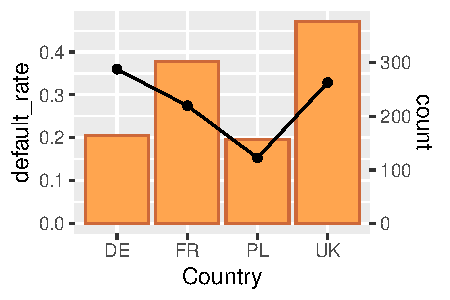
\includegraphics{Risk-Models-Development-Process_files/figure-beamer/unnamed-chunk-52-1.pdf}

\end{frame}

\begin{frame}[fragile]{Acceptance criteria - No counterintuitive signs}

\begin{verbatim}
##        Driver Sign Estimate
## 2 Industry_AB    +     0.79
\end{verbatim}

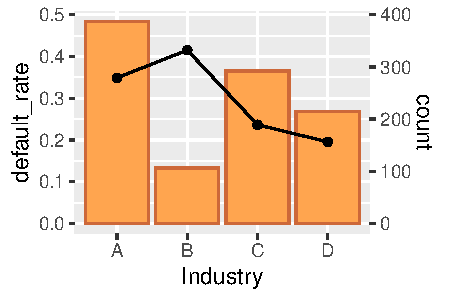
\includegraphics{Risk-Models-Development-Process_files/figure-beamer/unnamed-chunk-53-1.pdf}

\end{frame}

\begin{frame}[fragile]{Acceptance criteria - No counterintuitive signs}

\begin{verbatim}
##         Driver Sign Estimate
## 3 Total_assets    -    -0.12
\end{verbatim}

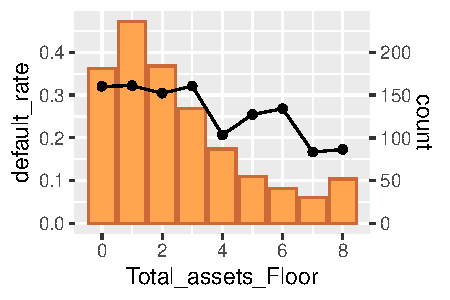
\includegraphics{Risk-Models-Development-Process_files/figure-beamer/unnamed-chunk-54-1.pdf}

\end{frame}

\begin{frame}[fragile]{Acceptance criteria - No counterintuitive signs}

\begin{verbatim}
##         Driver Sign Estimate
## 4 Credit_limit   -?     0.23
\end{verbatim}

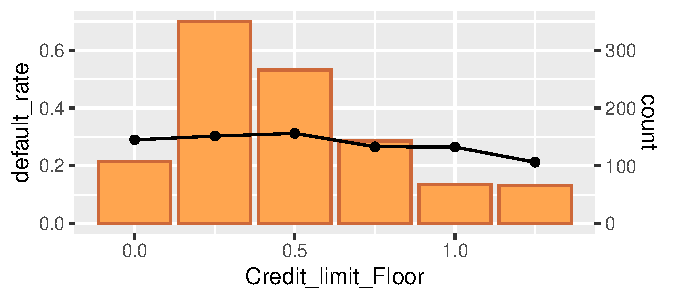
\includegraphics{Risk-Models-Development-Process_files/figure-beamer/unnamed-chunk-55-1.pdf}

\end{frame}

\begin{frame}[fragile]{Acceptance criteria - No counterintuitive signs}

\begin{verbatim}
##   Driver Sign Estimate
## 5    EDF   +?      -27
\end{verbatim}

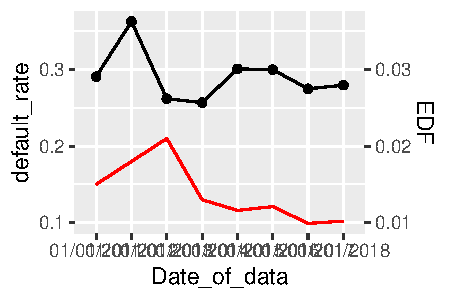
\includegraphics{Risk-Models-Development-Process_files/figure-beamer/unnamed-chunk-56-1.pdf}

\end{frame}

\begin{frame}[fragile]{Acceptance criteria - p-value}

\begin{Shaded}
\begin{Highlighting}[]
\NormalTok{summary <-}\StringTok{ }\KeywordTok{data.frame}\NormalTok{(}\KeywordTok{coef}\NormalTok{(}\KeywordTok{summary}\NormalTok{(m0))[,}\KeywordTok{c}\NormalTok{(}\DecValTok{1}\NormalTok{,}\DecValTok{4}\NormalTok{)])}
\NormalTok{summary}\OperatorTok{$}\NormalTok{p_val_less_5PRC <-}\StringTok{ }\NormalTok{summary[,}\DecValTok{2}\NormalTok{] }\OperatorTok{<=}\StringTok{ }\FloatTok{0.05}
\NormalTok{summary}
\end{Highlighting}
\end{Shaded}

\begin{verbatim}
##                 Estimate     Pr...z.. p_val_less_5PRC
## (Intercept)   -0.6016979 8.688847e-02           FALSE
## Country_PL    -0.9552921 2.426389e-04            TRUE
## Industry_AB    0.7913721 1.246686e-06            TRUE
## Total_assets  -0.1156390 1.328641e-02            TRUE
## Credit_limit   0.2254393 4.948075e-01           FALSE
## EDF          -26.7674014 2.067853e-01           FALSE
\end{verbatim}

\end{frame}

\begin{frame}[fragile]{Acceptance criteria - correlation}

No two variables can be correlated more than 0.50 in absolute terms.

\begin{Shaded}
\begin{Highlighting}[]
\NormalTok{corr_data <-}\StringTok{ }\KeywordTok{subset}\NormalTok{(development_sample,}
                    \DataTypeTok{select =} \KeywordTok{c}\NormalTok{(}\StringTok{"Country_PL"}\NormalTok{,}
                               \StringTok{"Industry_AB"}\NormalTok{,}
                               \StringTok{"Total_assets"}\NormalTok{,}
                               \StringTok{"Credit_limit"}\NormalTok{,}
                               \StringTok{"EDF"}\NormalTok{))}
\NormalTok{correlation_results <-}\StringTok{ }\KeywordTok{cor}\NormalTok{(corr_data)}
\end{Highlighting}
\end{Shaded}

\end{frame}

\begin{frame}[fragile]{Acceptance criteria - correlation}

\begin{verbatim}
##              Country_PL Industry_AB Total_assets
## Country_PL       1.0000      -0.027       0.0053
## Industry_AB     -0.0271       1.000       0.0123
## Total_assets     0.0053       0.012       1.0000
## Credit_limit     0.0193      -0.025       0.7145
## EDF             -0.0395       0.068      -0.0405
##              Credit_limit    EDF
## Country_PL          0.019 -0.040
## Industry_AB        -0.025  0.068
## Total_assets        0.715 -0.040
## Credit_limit        1.000 -0.028
## EDF                -0.028  1.000
\end{verbatim}

\end{frame}

\begin{frame}{Acceptance criteria - Summary}

\begin{itemize}
\tightlist
\item
  Expected sign

  \begin{itemize}
  \tightlist
  \item
    Credit\_limit and EDF do not meet the criteria
  \end{itemize}
\item
  Significance (p-value)

  \begin{itemize}
  \tightlist
  \item
    Credit\_limit and EDF do not meet the criteria
  \end{itemize}
\item
  Correlation

  \begin{itemize}
  \tightlist
  \item
    Total\_assets and Credit\_limit cannot appear in the same model
  \end{itemize}
\end{itemize}

Result -\textgreater{} model rejected

\end{frame}

\begin{frame}{Model search}

An estimation is done for each possible model and only the models that
fulfil all the criteria are considered further. In practice:

\begin{itemize}
\tightlist
\item
  models including correlated pairs of variables are not estimated
\item
  regulatory requirements state that some kinds of variables need to be
  included, eg:

  \begin{itemize}
  \tightlist
  \item
    customer size or proxy
  \item
    macroeconomic
  \end{itemize}
\end{itemize}

\end{frame}

\section{6. Model selection}\label{model-selection}

\begin{frame}{Model selection - performance criteria}

For all the models that passed the acceptance criteria we calculate some
performance metrics eg.:

\begin{itemize}
\tightlist
\item
  Gini coefficient - the higher the better
\item
  Akaike information criterion (AIC) - the lower the better
\end{itemize}

\end{frame}

\begin{frame}{AIC - Akaike Information Criteria}

\[ AIC = 2k - 2ln(\hat{L}),\] where:

\(k\) - number of parameters (penalize more parameters)

\(\hat{L}\) - likelihood function (promote higher likelihood)

\end{frame}

\begin{frame}{Model selection - performance criteria}

Let's compare three models:

\begin{itemize}
\tightlist
\item
  m1: Default \textasciitilde{} Industry\_AB + Length\_of\_business +
  Total\_assets
\item
  m2: Default \textasciitilde{} Country\_PL + Length\_of\_business +
  Total\_assets
\item
  m3: Default \textasciitilde{} Country\_PL + Industry\_AB +
  Length\_of\_business + Total\_assets
\end{itemize}

\end{frame}

\begin{frame}[fragile]{Model selection - estimation of parameters}

\begin{Shaded}
\begin{Highlighting}[]
\NormalTok{m1 <-}\StringTok{ }\KeywordTok{glm}\NormalTok{(}\DataTypeTok{data =}\NormalTok{ development_sample,}
          \DataTypeTok{formula =}\NormalTok{ Default }\OperatorTok{~}\StringTok{ }\NormalTok{Industry_AB }\OperatorTok{+}\StringTok{ }\NormalTok{Length_of_business }\OperatorTok{+}
\StringTok{                              }\NormalTok{Total_assets,}
          \DataTypeTok{family =}\NormalTok{ binomial)}
\NormalTok{m2 <-}\StringTok{ }\KeywordTok{glm}\NormalTok{(}\DataTypeTok{data =}\NormalTok{ development_sample,}
          \DataTypeTok{formula =}\NormalTok{ Default }\OperatorTok{~}\StringTok{ }\NormalTok{Country_PL }\OperatorTok{+}\StringTok{ }\NormalTok{Length_of_business }\OperatorTok{+}
\StringTok{                              }\NormalTok{Total_assets,}
          \DataTypeTok{family =}\NormalTok{ binomial)}
\NormalTok{m3 <-}\StringTok{ }\KeywordTok{glm}\NormalTok{(}\DataTypeTok{data =}\NormalTok{ development_sample,}
          \DataTypeTok{formula =}\NormalTok{ Default }\OperatorTok{~}\StringTok{ }\NormalTok{Country_PL }\OperatorTok{+}\StringTok{ }\NormalTok{Industry_AB }\OperatorTok{+}
\StringTok{                              }\NormalTok{Length_of_business }\OperatorTok{+}\StringTok{ }\NormalTok{Total_assets,}
          \DataTypeTok{family =}\NormalTok{ binomial)}
\end{Highlighting}
\end{Shaded}

\end{frame}

\begin{frame}[fragile]{Model selection - Gini}

We predict the probabilities for each model

\begin{Shaded}
\begin{Highlighting}[]
\NormalTok{development_sample}\OperatorTok{$}\NormalTok{prediction_m1 =}
\StringTok{              }\KeywordTok{fitted.values}\NormalTok{(m1)}
\NormalTok{development_sample}\OperatorTok{$}\NormalTok{prediction_m2 =}
\StringTok{              }\KeywordTok{fitted.values}\NormalTok{(m2)}
\NormalTok{development_sample}\OperatorTok{$}\NormalTok{prediction_m3 =}
\StringTok{              }\KeywordTok{fitted.values}\NormalTok{(m3)}
\end{Highlighting}
\end{Shaded}

\end{frame}

\begin{frame}[fragile]{Model selection - Gini}

\begin{Shaded}
\begin{Highlighting}[]
\KeywordTok{print}\NormalTok{(}\KeywordTok{head}\NormalTok{(}\KeywordTok{subset}\NormalTok{(development_sample, }\DataTypeTok{select =}
                    \KeywordTok{c}\NormalTok{(Default,prediction_m1,}
\NormalTok{                      prediction_m2,prediction_m3)),}
           \DecValTok{10}\NormalTok{),}\DataTypeTok{digits =} \DecValTok{2}\NormalTok{)}
\end{Highlighting}
\end{Shaded}

\begin{verbatim}
##    Default prediction_m1 prediction_m2 prediction_m3
## 1        1         0.406         0.357         0.440
## 2        0         0.043         0.071         0.048
## 4        1         0.237         0.202         0.259
## 5        0         0.235         0.207         0.255
## 6        1         0.297         0.259         0.324
## 8        0         0.390         0.343         0.423
## 9        0         0.311         0.269         0.339
## 10       0         0.331         0.463         0.365
## 12       0         0.195         0.293         0.218
## 13       0         0.568         0.283         0.357
\end{verbatim}

\end{frame}

\begin{frame}[fragile]{Model selection - Gini}

\begin{Shaded}
\begin{Highlighting}[]
\NormalTok{model_summary <-}\StringTok{ }\KeywordTok{data.frame}\NormalTok{(}
              \StringTok{"Model"}\NormalTok{=}\StringTok{ }\KeywordTok{c}\NormalTok{(}\StringTok{"m1"}\NormalTok{,}\StringTok{"m2"}\NormalTok{,}\StringTok{"m3"}\NormalTok{),}
              \StringTok{"Gini_development"}\NormalTok{ =}
\StringTok{                }\KeywordTok{c}\NormalTok{(}\KeywordTok{Gini}\NormalTok{(development_sample}\OperatorTok{$}\NormalTok{prediction_m1,}
\NormalTok{                        development_sample}\OperatorTok{$}\NormalTok{Default),}
                  \KeywordTok{Gini}\NormalTok{(development_sample}\OperatorTok{$}\NormalTok{prediction_m2,}
\NormalTok{                        development_sample}\OperatorTok{$}\NormalTok{Default),}
                  \KeywordTok{Gini}\NormalTok{(development_sample}\OperatorTok{$}\NormalTok{prediction_m3,}
\NormalTok{                        development_sample}\OperatorTok{$}\NormalTok{Default)))}
\end{Highlighting}
\end{Shaded}

\end{frame}

\begin{frame}[fragile]{Model selection - Gini}

\begin{Shaded}
\begin{Highlighting}[]
\KeywordTok{print}\NormalTok{(model_summary, }\DataTypeTok{digits =} \DecValTok{3}\NormalTok{)}
\end{Highlighting}
\end{Shaded}

\begin{verbatim}
##   Model Gini_development
## 1    m1            0.215
## 2    m2            0.195
## 3    m3            0.228
\end{verbatim}

\end{frame}

\begin{frame}[fragile]{Model selection - AIC}

\begin{Shaded}
\begin{Highlighting}[]
\NormalTok{model_summary}\OperatorTok{$}\NormalTok{AIC <-}\StringTok{ }\KeywordTok{c}\NormalTok{(}\KeywordTok{AIC}\NormalTok{(m1),}\KeywordTok{AIC}\NormalTok{(m2),}\KeywordTok{AIC}\NormalTok{(m3))}
\KeywordTok{print}\NormalTok{(model_summary, }\DataTypeTok{digits =} \DecValTok{3}\NormalTok{)}
\end{Highlighting}
\end{Shaded}

\begin{verbatim}
##   Model Gini_development AIC
## 1    m1            0.215 869
## 2    m2            0.195 872
## 3    m3            0.228 854
\end{verbatim}

\end{frame}

\begin{frame}{Model selection - Champion and Challenger}

After the analysis of all possible models for all functional forms
considered we choose:

\begin{itemize}
\tightlist
\item
  Champion model - best model (our m3)
\item
  Challenger model - second best (our m1)
\end{itemize}

\end{frame}

\section{7. Model validation}\label{model-validation}

\begin{frame}[fragile]{Model validation}

We need to check how our champion and challanger models perform on the
hold-out sample

\begin{Shaded}
\begin{Highlighting}[]
\NormalTok{hold_out_sample}\OperatorTok{$}\NormalTok{prediction_m3 <-}\KeywordTok{predict}\NormalTok{(m3,}
                      \DataTypeTok{newdata =}\NormalTok{ hold_out_sample, }\DataTypeTok{type =} \StringTok{'response'}\NormalTok{)}
\NormalTok{hold_out_sample}\OperatorTok{$}\NormalTok{prediction_m1 <-}\KeywordTok{predict}\NormalTok{(m1,}
                      \DataTypeTok{newdata =}\NormalTok{ hold_out_sample, }\DataTypeTok{type =} \StringTok{'response'}\NormalTok{)}
\end{Highlighting}
\end{Shaded}

\end{frame}

\begin{frame}[fragile]{Validation - Gini}

\begin{Shaded}
\begin{Highlighting}[]
\NormalTok{validation_summary <-}\StringTok{ }\KeywordTok{data.frame}\NormalTok{(}
              \StringTok{"Model"}\NormalTok{=}\StringTok{ }\KeywordTok{c}\NormalTok{(}\StringTok{"m3"}\NormalTok{,}\StringTok{"m1"}\NormalTok{),}
              \StringTok{"Gini_hold_out"}\NormalTok{ =}
\StringTok{                }\KeywordTok{c}\NormalTok{(}\KeywordTok{Gini}\NormalTok{(hold_out_sample}\OperatorTok{$}\NormalTok{prediction_m3,}
\NormalTok{                      hold_out_sample}\OperatorTok{$}\NormalTok{Default),}
                  \KeywordTok{Gini}\NormalTok{(hold_out_sample}\OperatorTok{$}\NormalTok{prediction_m1,}
\NormalTok{                      hold_out_sample}\OperatorTok{$}\NormalTok{Default)))}
\end{Highlighting}
\end{Shaded}

\end{frame}

\begin{frame}[fragile]{Validation - Gini}

\begin{Shaded}
\begin{Highlighting}[]
\KeywordTok{print}\NormalTok{(validation_summary, }\DataTypeTok{digits =} \DecValTok{3}\NormalTok{)}
\end{Highlighting}
\end{Shaded}

\begin{verbatim}
##   Model Gini_hold_out
## 1    m3         0.235
## 2    m1         0.232
\end{verbatim}

\end{frame}

\begin{frame}[fragile]{Summarize}

\begin{Shaded}
\begin{Highlighting}[]
\NormalTok{summary_final <-}\StringTok{ }\KeywordTok{merge}\NormalTok{(}\DataTypeTok{x =}\NormalTok{ model_summary,}
                       \DataTypeTok{y =}\NormalTok{ validation_summary,}
                       \DataTypeTok{by =} \StringTok{"Model"}\NormalTok{,}
                       \DataTypeTok{all.y =} \OtherTok{TRUE}\NormalTok{) }\OperatorTok\StringTok{ }\KeywordTok{subset}\NormalTok{(}\DataTypeTok{select=}\OperatorTok{-}\KeywordTok{c}\NormalTok{(AIC))}
\NormalTok{summary_final}\OperatorTok{$}\NormalTok{Dev_minus_hold_out <-}
\StringTok{  }\NormalTok{summary_final}\OperatorTok{$}\NormalTok{Gini_development }\OperatorTok{-}\StringTok{ }\NormalTok{summary_final}\OperatorTok{$}\NormalTok{Gini_hold_out}
\end{Highlighting}
\end{Shaded}

\end{frame}

\begin{frame}[fragile]{Summarize}

\begin{Shaded}
\begin{Highlighting}[]
\KeywordTok{print}\NormalTok{(summary_final, }\DataTypeTok{digits =} \DecValTok{3}\NormalTok{)}
\end{Highlighting}
\end{Shaded}

\begin{verbatim}
##   Model Gini_development Gini_hold_out Dev_minus_hold_out
## 1    m1            0.215         0.232            -0.0173
## 2    m3            0.228         0.235            -0.0063
\end{verbatim}

\end{frame}

\begin{frame}[fragile]{Conclusions}

\begin{itemize}
\tightlist
\item
  Both models seem to perform better on the hold-out sample than on the
  development sample
\item
  The classification remains the same:

  \begin{itemize}
  \tightlist
  \item
    Champion: m3 - Default \textasciitilde{} Country\_PL + Industry\_AB
    + Length\_of\_business + Total\_assets
  \end{itemize}
\end{itemize}

\begin{Shaded}
\begin{Highlighting}[]
\KeywordTok{print}\NormalTok{(}\KeywordTok{coefficients}\NormalTok{(m3), }\DataTypeTok{digits =} \DecValTok{3}\NormalTok{)}
\end{Highlighting}
\end{Shaded}

\begin{verbatim}
##        (Intercept)         Country_PL        Industry_AB 
##             0.3462            -1.0112             0.7339 
## Length_of_business       Total_assets 
##            -0.2759            -0.0955
\end{verbatim}

\end{frame}

\begin{frame}[fragile]{Conclusions}

\begin{itemize}
\tightlist
\item
  Challenger: m1 - Default \textasciitilde{} Industry\_AB +
  Length\_of\_business + Total\_assets
\end{itemize}

\begin{Shaded}
\begin{Highlighting}[]
\KeywordTok{print}\NormalTok{(}\KeywordTok{coefficients}\NormalTok{(m1), }\DataTypeTok{digits =} \DecValTok{3}\NormalTok{)}
\end{Highlighting}
\end{Shaded}

\begin{verbatim}
##        (Intercept)        Industry_AB Length_of_business 
##             0.1781             0.7392            -0.2712 
##       Total_assets 
##            -0.0927
\end{verbatim}

\end{frame}

\begin{frame}{End}

------------------------------------ THANK YOU!!!
------------------------------------

\end{frame}

\end{document}
